\chapter{绪论}
\label{chap:introduction}

\section{研究背景和意义}
核磁共振成像\cite{mrireview}(magnetic resonance imaging, MRI)是临床上常用的成像方式,如图\ref{fig:mri}所示。
\begin{figure}[htbp]
\centerline{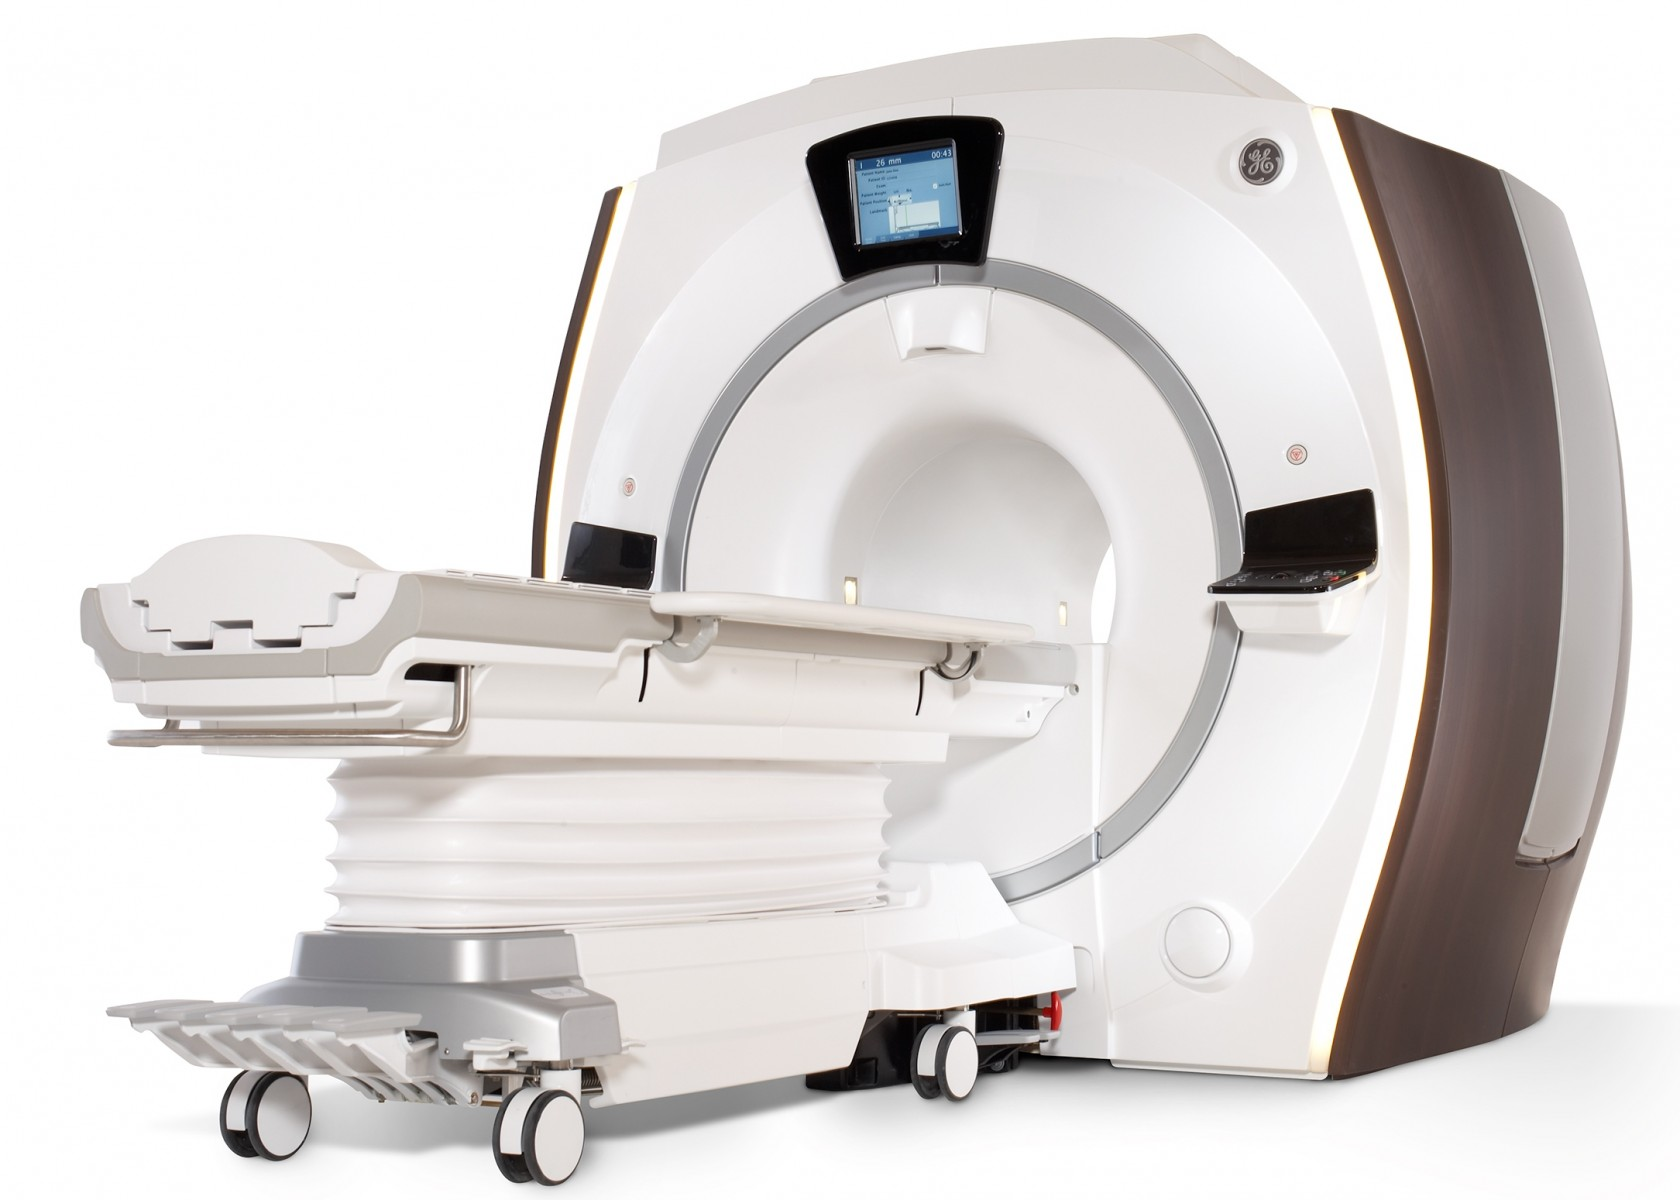
\includegraphics[width=0.7\textwidth]{img/intro/mri.jpg}}
\caption{MR成像设备。}
\label{fig:mri}
\end{figure}
MRI利用核磁共振现象来实现高对比度成像,它可以非侵入式地获取人体内部组织信息,广泛地应用于指导病灶检测、诊断与治疗。MRI在临床和研究中有很多不同的分类方式,根据是否含有时间维度,可以将MR图像分为静态MR图像和动态MR图像(dynamic MRI,dMRI)。常见的动态MRI有心脏电影成像(cardiac cine)、心脏灌注成像(cardiac perfusion)、磁共振动态对比增强(dynamic contrast enhanced MRI,DCE-MRI)、功能核磁共振成像(function MRI,fMRI)等,如图\ref{fig:dynamic}所示。
\begin{figure}[htbp]
\centering
\subfigure[心脏电影(一帧)]{
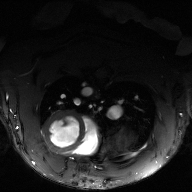
\includegraphics[width=2.11in]{img/intro/cine.png}
}
\subfigure[胸部DCE-MRI(一帧)]{
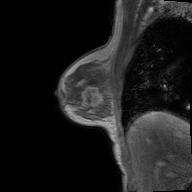
\includegraphics[width=2.11in]{img/intro/breast.png}
}
\subfigure[心脏灌注(一帧)]{
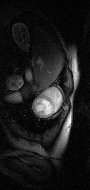
\includegraphics[width=1in]{img/intro/perfusion.png}
}
\centering
\caption{动态MR图像举例。}
\label{fig:dynamic}
\end{figure}
根据研究方法的不同,可以将MRI分为定性(qualitative)MRI和定量MRI(quantitative MRI,qMRI),如图\ref{fig:qvsq}所示。
\begin{figure}[htbp]
\centering
\subfigure[$T_1$加权图像]{
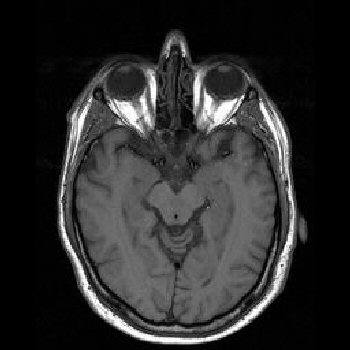
\includegraphics[width=2.5in]{img/intro/t1w.jpg}
}
\subfigure[$T_2$加权图像]{
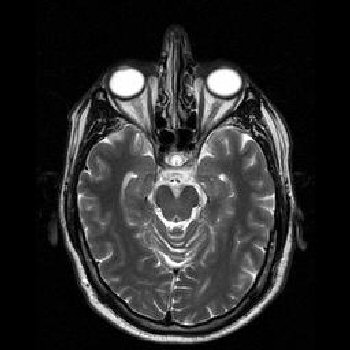
\includegraphics[width=2.5in]{img/intro/t2w.jpg}
}

\subfigure[$T_1$图像]{
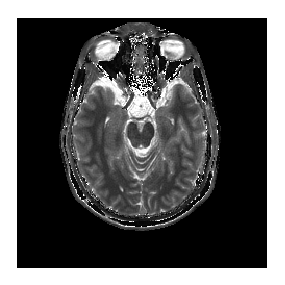
\includegraphics[width=2.5in]{img/intro/t1.eps}
}
\subfigure[$T_2$图像]{
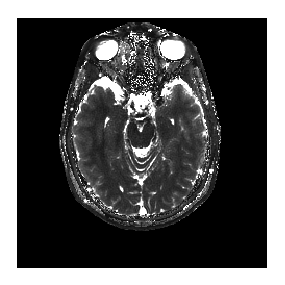
\includegraphics[width=2.5in]{img/intro/t2.eps}
}
\centering
\caption{定性MR图像与定量MR图像。}
\label{fig:qvsq}
\end{figure}
定性MR图像是临床诊断中最常用到的类型,如$T_1$加权图像和$T_2$加权图像等,其对比度的来源分别为组织$T_1$和$T_2$的差异。因此其像素值大小只是反映了$T_1$和$T_2$大小,并不是$T_1$和$T_2$本身。通过定性MR图像进行的诊断主要依靠医生的主观认识,缺乏定量指标。而定量MRI不仅能够提供组织的基本结构,也能获得组织的定量参数,从而减少了主观性,从客观定量的角度研究人体组织,达到帮助诊断与评估治疗的作用。DCE-MRI\cite{Yankeelov2009}是定量MRI的重要应用,被成功应用在胸部肿瘤定量分析以及脑灌注成像中。DCE-MRI是通过注入对比剂引起的信号改变以评估组织灌注以及为血管通透性,常见的量化参数有体积转移常数($K^{trans}$)和血管外细胞体积分数($v_e$)等。我们将在第\ref{chap:qetsr}章中介绍并讨论胸部DCE-MRI的重建。磁共振指纹\cite{mrf}(magnetic resonance fingerprinting,MRF)是近年来qMRI中的研究热点,可以同时快速获得多个组织参数,并且重建的定量参数图有很高的信噪比。MRF重建的过程主要包括预定义字典的生成、信号采集和模式识别三个部分。具体来说,给定一个MR序列,首先使用数学模型生成一个包含不同参数的组织体素在该MR序列中的演化过程的字典,然后将采集到的信号与字典中的原子进行匹配,从而获得该体素的组织参数。我们将分别在第\ref{sec:mrf}章介绍MRF的研究现状。

MR成像过程通常被建模为二维或三维空间的Fourier编码,即首先从图像的Fourier域(通常称为k-space)中采样,再通过算法将图像重建出来。详细的MR成像原理请参考第\ref{chap:pre}章。为了准确地重建图像,采样率需要达到Nyquist采样定理\cite{Nyquist}的要求。所以,MRI的成像速度通常很慢,尤其是dMRI和三维MRI,这对成像设备和病人都是很大的负担。因此如何提高MR成像速度和质量,一直是研究人员最关心的问题。

加速MR成像通常的思路是在不降低图像质量的前提下,减少获取的k-space数据,从而达到加速成像的效果。但由于下采样时,采样率没有达到Nyquist采样定理的要求,通过简单的Fourier补零重建的图像(称为Zerofilled图像)会出现下采样伪影,而消除伪影主要有以下三个策略。第一种策略是使得生成的伪影与图像非相干或者在视觉上不明显\cite{Tsai,Marseille,Greiser},但这些方法所得到的重建图像通常信噪比低。第二种策略是利用k-space中数据的冗余性,比如部分傅里叶成像\cite{McGibney}(partial-Fourier)和平行成像(parallel MRI, pMRI)。pMRI是目前在临床上应用比较成功的一大类加速方法,它是一种以空间换时间的成像策略。具体来说,pMRI通过多个成像线圈接收信号,而每个线圈都在k-space进行下采样,最后通过算法将所有线圈接收到的数据还原出来。经典的pMRI方法有SENSE(sensitivity encoding)\cite{sense},SMASH(simultaneous acquisition of spatial harmonics)\cite{smash},GRAPPA(generalized autocalibrating partially parallel acquisitions)\cite{grappa}等。第三种策略是利用图像在空间域或者时间域上的冗余性,如UNFOLD\cite{Madore}和k-t BLAST/SNESE\cite{Tsao}等。可以看出,以上方法的共同点是假设MR图像中存在着冗余性,并且可以利用这些冗余性来降低采样率,以达到加速成像的目的。

2005年,Candès,Tao,Romberg\cite{candes2004near,candes2006compressive,candes2006quantitative,candes2006stable}和Donoho\cite{Donoho2006Compressed}等人提出了压缩感知(compressed sensing)理论。压缩感知是一种新的采样理论,可以加速信号的采集与重建。根据传统Nyquist采样定理\cite{Nyquist},当采样率达到信号最高频率两倍以上的时,信号才可以被精确地重建出来。我们称满足Nyquist采用定理的采样方式成为全采样。当对信号进行均匀下采样时,采集到的信号会出现相干伪影,使用传统的重建方法很难将其去除。而压缩感知理论突破了Nyquist定理对高采样率要求的限制,可以用很少的数据来精确地重建信号。压缩感知理论有三个主要部分,分别为稀疏性、非相干下采样和非线性重建算法。具体来说,首先假设信号在某个变换域稀疏,对信号进行非相干下采样,然后通过非线性重建算法即可以高概率地将信号重建出来。因此,压缩感知理论自诞生以来就被应用在MR成像中,可以显著地提高成像速度和质量,并成为了快速MR成像的主流方法。本论文研究的重点之一即为压缩感知在MRI中的应用,我们将在第\ref{sec:cs}和\ref{sec:csmri}小节介绍基于压缩感知的MR成像的研究现状。

\section{压缩感知的基本理论}
\label{sec:cs}
我们首先介绍压缩感知的基本理论和基本模型。压缩感知理论是Candès,Romberg,Tao\cite{candes2004near,candes2006compressive,candes2006quantitative,candes2006stable}和Donoho\cite{Donoho2006Compressed}等提出的采样理论。数学上,压缩感知理论表明旨在求解以下欠定模型:
\begin{equation}
	b=Ax+\epsilon,
	\label{equ:cs}
\end{equation}
其中$x\in \mathbb{C}^N$,$A\in \mathbb{C}^{M\times N}$,$b\in \mathbb{C}^M$,$\epsilon\in \mathbb{C}^N$,$M<<N$。压缩感知的过程即是从$b$重建$x$的过程,在数学上被称为反问题。反问题在现实中有着广泛的应用,比如医学成像\cite{golbabaee2012hyperspectral,quinsac2010compressed,xu2012low,lustig2006}、计算机视觉\cite{wright2008robust}、雷达成像\cite{choi2010compressed}等。在MR成像中,$A$通常被称作采样矩阵,$x$为需要恢复的图像,$b$是测量的到的k-space数据,$\epsilon$为测量噪声。由于$M<<N$,这个问题是病态的,所以我们需要对$x$有所约束。

\subsection{稀疏性}
压缩感知理论先验性地假设信号本身或者在某个变换域下是稀疏的。稀疏性是信号的固有属性,实际生活中的信号,如声音、图像、视频等一般在某个变化域下的系数都是稀疏的或者近似稀疏的。比如,分片常数的图像在梯度域中是稀疏的,而分片光滑的图像在小波变换域中是近似稀疏的。

在数学上,称向量$x\in \mathbb{C}^N$为$s$-稀疏的,如果
\begin{equation}
	\|x\|_0 \leq s.
\end{equation}
这里$s<N$,$\|x\|_0$为$x$的$l_0$范数,其定义为
$$\|x\|_0=|\mathrm{supp(x)}|,\quad \mathrm{supp}(x)=\{j: x_j\neq 0\},$$
即$x$的$l_0$范数为$x$中非零元素的个数。对于$s\in \{1,2,...,N\}$,我们记
$$\Sigma_s=\{x\in\mathbb{C}^N: \|x\|_0\leq s\}$$
为$s$-稀疏向量的集合。进一步,$x\in \mathbb{C}^N$的最佳$s$项近似误差为:
$$\sigma_s(x)_p=\mathrm{inf}_{z\in \Sigma_s}\|x-z\|_p.$$
如果$\sigma_s(x)$在$s$项内衰减很快,则称$x$为可压缩的。可以看出,可压缩向量可以由稀疏向量近似得到。这里向量$x$的$p$范数的定义为:
\begin{equation}
	\|x\|_p = (\sum_{j=1}^N|x_n|^p)^{1/p},\quad 0<p<\infty.
\end{equation}
在实际中,信号本身很少是真正稀疏的或者可压缩的,而是在某个变换域下是稀疏的或者可压缩的。常用的稀疏变化有正交变换、Fourier变换、小波变换、紧框架、字典学习等。

\subsection{采样矩阵}
压缩感知重建模型旨在寻找模型(\ref{equ:cs})最稀疏的解。数学上,这个过程可以描述为以下约束优化问题:
\begin{equation}
\begin{aligned}
	\hat{x}&=\argmin_x \|x\|_0,\\
	&s.t.\quad \|Ax-b\|_2^2 \leq \epsilon.
\end{aligned}
\label{equ:l0}
\end{equation}
我们通常称这个问题为P0问题。但是由于(\ref{equ:l0})非凸的,而且是NP难的,直接求解计算量很大。通常的求解方法有贪婪算法\cite{cosamp,tropp2006just}、重新加权范数算法\cite{gorodnitsky1997sparse,candes2008enhancing}、凸松弛法\cite{chen2001atomic}等。其中$l_1$范数凸松弛方法是最常用的方法,其旨在解决以下优化问题:
\begin{equation}
\begin{aligned}
	\hat{x}&=\argmin_x \|x\|_1,\\
	&s.t.\quad \|Ax-b\|_2^2 \leq \epsilon.
\end{aligned}
\label{equ:l1}
\end{equation}
$l_1$优化问题也被称为基追踪(basic pursuit\cite{bp})和P1问题。

为了保证压缩感知重建的精确性和鲁棒性,采样矩阵$A$需要满足特定的性质。压缩感知理论目前给出的性质有三个,它们分别为零空间性质(null space property,NSP),等距约束性(restricted isometry property, RIP)和非相干性(incoherence)。其中零空间性质是$l_1$优化分析中的基本性质,其定义为:

\noindent\textbf{定义 1.2.2.1} 称矩阵$A\in \mathbb{C}^{M\times N}$满足$s$-零空间性质,如果
$$\|\eta_\mathcal{O}\|_1\leq \gamma\|\eta_{\mathcal{O}^c}\|_1$$
对于所有集合$\mathcal{O}\subset\{1,...,N\},\#\mathcal{O}\leq s$和所有$\eta\in \mathrm{ker}A=\{x|Ax=0\}$均成立。其中,$\eta_\mathcal{O}$为下标与集合$\mathcal{O}$中元素一致的向量,$\mathcal{O}^c$为集合$\mathcal{O}$的补集,$\#\mathcal{O}$为集合$\mathcal{O}$中元素的个数,$\gamma\in (0,1)$为常数。以下的定理保证了P1问题解的存在性。

\noindent\textbf{定理 1.2.2.2} 设$A\in \mathbb{C}^{M\times N}$满足$s$-零空间性质。令$x\in \mathbb{C}^N$,$b=Ax$并且$\hat{x}$是P1问题的解。那么如果$x$是$s$-稀疏的,则$\hat{x}=x$。

可以看出,零空间性质实际上等价于$l_1$稀疏重建。虽然NSP有着很好的性质,但在实际中很难判断一个采样矩阵是否满足零空间性质。而等距约束性更加容易处理,并且对噪声有鲁棒性。其定义如下:

\noindent\textbf{定义 1.2.2.3} 称采样矩阵$A\in \mathbb{C}^{M\times N}$具有$s$-等距约束性,如果存在最小的常数$0\leq\delta_s<0$使得
\begin{equation}
	(1-\delta_s)\|x\|_2^2\leq \|Ax\|_2^2\leq (1+\delta_s)\|x\|^2_2
\end{equation}
对所有$s$-稀疏信号成立。

矩阵的等距约束性本质上要求矩阵$A$的所有$M\times s$子矩阵接近等距,即稀疏信号从高维空间向低维空间投影时的距离保持不变。从等距约束性可以推导出一些充分条件保证压缩感知可以求解P1问题。比如,在没有噪声干扰的情况下,如果$\delta_{2s}<1$,P0问题有唯一的$s$-稀疏解存在;如果$\delta_{2s}<\sqrt{2}-1$,P1问题的解和等价于P0问题的解。当有噪声存在时,以下定理保证了P1问题解的存在性。

\noindent\textbf{定理 1.2.2.4} 假设$\delta_{2s}<\sqrt{2}-1$,则P1问题的解满足
$$\|\hat{x}-x\|_2\leq c_0s^{-1/2}\sigma_s(x)_1+c_1\epsilon,$$
其中$c_0$和$c_1$是与$\delta_{2s}$有关的大于零的常数。

虽然等距约束性在理论上给出了采样矩阵$A$需要满足的条件,但是在实际应用中,等距约束性不容易计算,因此很难验证一个采样矩阵是否具有等距约束性。非相干性则给采样矩阵的验证提供了简单有效的方法,其定义为:

\noindent\textbf{定义 1.2.2.5} 
矩阵$A$的列相干性为$A$中任意不同两列$a_i$与$a_j$内积的最大值:
\begin{equation}
	\mu(A) = \max_{i\neq j}\frac{|\langle a_i,a_j\rangle|}{\|a_i\|_2\|a_j\|_2}.
\end{equation}
可以看出,矩阵列相干性的范围是$\mu(A)\in [\sqrt{\frac{N-M}{M(N-1)}},1]$。

压缩感知理论表明,当采样矩阵$A$的列相干性接近于1时,压缩感知只需要$O(s\mathrm{log}N)$次测量就可以很大概率恢复出原信号。

\subsection{非线性重建算法}
在实际计算中,我们一般将问题(\ref{equ:l1})转化成更容易处理的无约束问题求解,模型变为:
\begin{equation}
	\hat{x}=\argmin_x \|Ax-b\|_2^2 + \alpha\|x\|_1.
	\label{equ:unconstraint}
\end{equation}
其中$\alpha$是与噪声相关参数。可以看出,问题(\ref{equ:unconstraint})是凸的,但不可微。目前有很多快速算法来求解优化问题(\ref{equ:unconstraint}),有关算法的详细信息请参考文献\cite{proximal}。这些算法可以分为两类,一类是内点方法,另一类是一阶算法。一阶算法通常比内点算法计算更简便,也更适合处理大规模数据的情形。因此本文主要考虑一阶算法。

常用的一阶重建算法有向前向后分裂算法(forward-backward splitting\cite{fbs}, FBS),分裂Bregman迭代算法(split Bregman\cite{sb}),交替方向法(alternating directional method of multiplier\cite{admm,ramani2010parallel,boyd2011distributed,yang2011alternating}, ADMM),Douglas-Rachford分裂算法\cite{dr},快速阈值收缩算法(fast iterative shrinkage threshold algorithm\cite{fista}, FISTA),主对偶算法(Primal-Dual\cite{pd})等。其中ADMM算法最先被应用在压缩感知的重建中,也是最早被应用于MR压缩感知重建的算法之一。ADMM算法通过算子分裂将问题(\ref{equ:unconstraint})转化为如下约束优化问题:
\begin{equation}
\begin{aligned}
	&\hat{x}=\argmin_x \|Ax-b\|_2^2 + \alpha\|u\|_1,\\
	& s.t. \quad u=x.
\end{aligned}
\label{equ:admm}
\end{equation}
问题(\ref{equ:admm})的增广Lagrangian形式为:
\begin{equation}
	L_\mu(x,u,v)=\|Ax-b\|^2_2+\alpha\|u\|_1+\langle v,u-x\rangle +\frac{\mu}{2}\|u-x\|_2^2.
\label{equ:admm2}
\end{equation}
通过交替方向法求解问题(\ref{equ:admm2}),其迭代步骤为:
\begin{equation}
	\begin{aligned}
		& u^{n+1}=\argmin_u L_\mu(x^n,u,v^n),\\
		& x^{n+1}=\argmin_x L_\mu(x,u^{n+1},v^n),\\
		& v^{n+1}=\argmin_v L_\mu(x^{n+1},u^{n+1},v).
	\end{aligned}
	\label{equ:admm3}
\end{equation}
可以看出,$l_1$重建的ADMM算法需要求解三个子问题。其中求解$u$子问题等价于求解
$$u^{n+1}=\argmin_u \frac{\mu}{2}\|u-x^n+\frac{1}{\mu}v^n\|_2^2+\alpha\|u\|_1,$$
可以使用软阈值收缩算法(soft-shrinkage)求解,其定义为:
$$\mathscr{S}_\lambda(t)=\frac{t}{|t|}\mathrm{max}\{|t|-\lambda,0\}.$$
取$t=x^n-\frac{1}{\mu}y^{n}$,$\lambda=\frac{\alpha}{\mu}$,则$u$子问题的解为:
\begin{equation}
	u^{n+1}=\mathscr{S}_\lambda(t).
	\label{equ:admmu}
\end{equation}
求解$x$子问题等价于求解
\begin{equation}
	x^{n+1}=\argmin_x \|Ax-b\|^2_2+\frac{\mu}{2}\|v-x^n+\frac{1}{\mu}v^n\|_2^2,
	\label{equ:admmx}
\end{equation}
可以通过共轭梯度算法\cite{powell1977restart}(conjugate gradient)进行求解。最后,$v$子问题即更新Lagrangian乘子为:
\begin{equation}
	v^{n+1}=v^{n}+\mu(u^{n+1}-x^{n+1}).
\end{equation}
于是$l_1$稀疏重建的ADMM算法的详细流程如算法\ref{alg:admm}所示。
\begin{algorithm}
	\caption{$l_1$稀疏重建模型的ADMM算法}
	\label{alg:admm}
	\begin{algorithmic}
		\REQUIRE $x^0, u^0, v^0$;
		\INDSTATE[-1.25] \textbf{迭代:根据以下步骤更新参数:}	
		\STATE 1.通过软阈值收缩算法求解(\ref{equ:admmu})更新$u^{n+1}$;
		\STATE 2.通过共轭梯度法求解(\ref{equ:admmx})更新$x^{n+1}$;
		\STATE 3. $v^{n+1}=v^{n}+\mu(u^{n+1}-x^{n+1})$;
		\ENSURE $x^{n+1}$。
	\end{algorithmic}
\end{algorithm}

ADMM算法是压缩感知的常用算法,但一方面由于ADMM算法需要使用共轭梯度法求解子问题,计算量大;另一方面ADMM算法参数多,调参的过程比较繁琐。FISTA\cite{fista}是也是压缩感知中常用算法,收敛速度快,而且需要调节的参数比ADMM少很多。FISTA算法考虑极小化下面的问题:
\begin{equation}
	\min_x\ f(x)+g(x),x\in \mathbb{C}^N,
\end{equation}
其中$f(x)$是凸的光滑函数,其Lipschitz常数为$L_f$,$g(x)$为凸函数,可能是非光滑的。定义连续凸函数$g(x)$的临近点算子:
\begin{equation}
	\mathrm{prox}_\tau(g)(x)=\argmin_u g(u)+\frac{1}{2\tau}\|u-x\|^2_2.
\end{equation}
则FISTA的算法流程如算法\ref{alg:fista}所示。
\begin{algorithm}
	\caption{FISTA算法迭代流程}
	\label{alg:fista}
	\begin{algorithmic}
		\REQUIRE $\tau = 1/L_f, t^1=1, x^0=r^1$;
		\INDSTATE[-1.25] \textbf{迭代:根据以下步骤更新参数:}	
		\STATE 1. $\bar{x}=r^k-\tau\nabla f(x^n)$;
		\STATE 2. $x^n=\prox_{\tau}(g)(\bar{x})$;
		\STATE 3. $t^{n+1}=(1+\sqrt{1+4(t^n)^2})/2$;
		\STATE 4. $r^{n+1}=x^n+\frac{t^n-1}{t^{n+1}}(x^n-x^{n-1})$;
		\ENSURE $x^{n+1}$。
	\end{algorithmic}
\end{algorithm}

将FISTA算法应用到问题(\ref{equ:unconstraint})中,令$f(x)=\|Ax-b\|^2_2$,$g(x)=\alpha\|x\|_1$,则$l_1$稀疏重建的FISTA算法流程如算法\ref{alg:fista2}所示。
\begin{algorithm}
	\caption{$l_1$稀疏重建的FISTA算法}
	\label{alg:fista2}
	\begin{algorithmic}
		\REQUIRE $\tau = 1/L_f, t^1=1, x^0=r^1$;
		\INDSTATE[-1.25] \textbf{迭代:根据以下步骤更新参数:}	
		\STATE 1. $\bar{x}=r^n-2\tau A^H(Ax-b)$;
		\STATE 2. $x^n=\prox_{\tau}(g)(\bar{x})$;
		\STATE 3. $t^{n+1}=(1+\sqrt{1+4(t^n)^2})/2$;
		\STATE 4. $r^{n+1}=x^n+\frac{t^n-1}{t^{n+1}}(x^n-x^{n-1})$;
		\ENSURE $x^{n+1}$。
	\end{algorithmic}
\end{algorithm}
FISTA算法是压缩感知重建中常用的算子分裂算法之一,被广泛应用于信号处理\cite{beck2009fast}和多任务学习\cite{ji2009accelerated}中。但是FISTA只能解决比较简单的模型,不能应用在含有多个正则项的模型中。我们将在第\ref{chap:qetsr}章中重点讨论和应用FISTA算法。

Primal-Dual\cite{pd}算法是近年来比较热门的一阶算法,收敛速度快,并且算法的收敛有着严格的定理保证。Primal-Dual算法被广泛应用于凸-凹鞍点问题的极大极小问题中:
\beq
\min_{x\in\mathcal{X}}\max_{y\in\mathcal{Y}}\quad\langle \mathcal{K}x,y\rangle+f(x)-g(y),
\label{equ:saddle1}
\eeq
其中$\mathcal{X}$和$\mathcal{Y}$是Hilbert空间,$\mathcal{K}:\mathcal{X}\rightarrow\mathcal{Y}$是线性连续映射,并且泛函$f:\mathcal{X}\rightarrow(-\infty,\infty]$和$g:\mathcal{Y}\rightarrow(-\infty,\infty]$是适定的、凸的和下半连续的。这里我们仅给出$l_1$稀疏优化问题(\ref{equ:unconstraint})的Primal-Dual算法的迭代步骤,如算法\ref{alg:primaldual}所示。具体的推导过程和详细信息请参考第\ref{chap:tgvlr}章。
\begin{algorithm}
	\caption{$l_1$稀疏重建的Primal-Dual算法}
	\label{alg:primaldual}
	\begin{algorithmic}
		\REQUIRE 选择$\tau, \sigma>0$,$x^0,y^0,p^0$,令$\bar{x}^0=x^0$;
		\INDSTATE[-1.25] \textbf{迭代:根据以下步骤更新参数:}	
		\STATE 1. $p^{n+1}=\mathcal{P}_\alpha(p^n+\sigma\bar{x}^n)$;
		\STATE 2. $r^{n+1}=[r^n+\sigma(A\bar{x}^n-b)]/(1+\sigma)$;
		\STATE 3. $x^{n+1}=x^n-\tau A^Hp^n$;
		\STATE 4. $\bar{x}^{n+1}=2x^{n+1}-x^n$;
		\ENSURE $x^{n+1}$。
	\end{algorithmic}
\end{algorithm}

\subsection{本节小结}
在本节中,我们回顾了压缩感知的数学模型和理论基础。压缩感知有三个主要部分,分别为稀疏性、采样矩阵和非线性重建算法。其中稀疏性是先验信息,采样矩阵保证了压缩感知重建模型解的存在性,而非线性重建算法决定了重建算法的速度的精度。

\section{基于压缩感知MR重建的研究现状}
\label{sec:csmri}
MR成像是从Fourier域(也称为k-space)采样并重建数据的过程。由于MR成像的固有时间长,如何加快成像速度一直是研究人员关心的话题。压缩感知理论为从欠采样数据中精确重建出MR图像提供了理论基础和算法框架。压缩感知理论表明,在假设MR图像在某个变换域稀疏的前提下,当采样矩阵满足等距约束性或者非相干性条件时\cite{Donoho2006Compressed},利用非线性重建算法可以大概率将图像精确地重建出来。压缩感知理论和MR成像有着天然的契合。为了使得压缩感知理论能够应用于MR成像,我们首先需要为MR图像找到合适的稀疏表示,并且采样矩阵也需要跟MR的成像域,即Fourier域非相干。在这一节中,我们重点回顾压缩感知在MR成像中的应用,MR成像原理请见第\ref{chap:pre}章。

\subsection{MR图像的稀疏性}
\label{sec:sparsity}
一般来说,医学图像是分片光滑的,因此在合适的稀疏变化下,医学图像通常展现出稀疏性或可压缩性。对于MR图像而言,其稀疏性或者说冗余性主要体现在三个方面。

第一,空间上的冗余性。自然图像通常在小波变换域或者有限差分域是稀疏的,因此小波变换和TV泛函被广泛应用与图像去噪和重建中。受此启发,Lustig\cite{lustig2006}通过实验验证了二维MR图像本身很少是稀疏的,但是其在小波变换域或者有限差分域上是稀疏的。图\ref{fig:wandtv}展示了体模图像在小波变换和有限差分下的稀疏性。可以看出,体模图像本身并不是稀疏的,但在小波变换和有限差分域下均体现出稀疏性,因此它们是基于压缩感知的MR重建模型中最常用的稀疏项。文献\cite{lustig2006}是从压缩感知理论的角度研究MR图像稀疏性的第一篇文献,之后的文献均从这个想法出发,根据具体问题提出不同的稀疏项,比如TGV(total generalized variation)\cite{tgv}、Shearlet\cite{easley2008sparse}、字典学习\cite{ksvd}等。

\begin{figure}[htbp]
\centering
\subfigure[体模图像]{
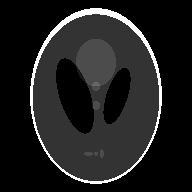
\includegraphics[width=2.5in]{img/intro/phantom.png}
}
\subfigure[一阶Haar小波变换]{
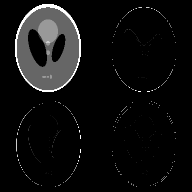
\includegraphics[width=2.5in]{img/intro/wavelet.png}
}

\subfigure[$x$方向的有限差分]{
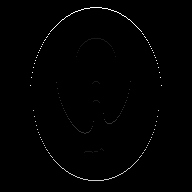
\includegraphics[width=2.5in]{img/intro/tvx.png}
}
\subfigure[$y$方向的有限差分]{
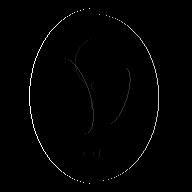
\includegraphics[width=2.5in]{img/intro/tvy.png}
}
\centering
\caption{体模图像稀疏性举例。}
\label{fig:wandtv}
\end{figure}


第二,时间上的冗余性。对于动态MR图像而言,其稀疏性不仅体现在空间方向上,也体现在时间方向上。动态MRI是MRI的重要应用之一,主要的应用有心脏电影成像、磁共振动态对比增强、功能磁共振成像等。动态MR常用的稀疏表示有Fourier变换、核范数、有限差分、字典学习等。比如,Lustig\cite{lustig2006}将一维Fourier变换作为时间方向上的稀疏项,并将模型应用在心脏电影成像中。其想法是,心脏作着周期性的运动,而Fourier变换可以稀疏化周期性的信号。但是在实际应用中,心脏的运动并不是完美的周期性,Fourier变换可能不是最优的选择。因此,基于数据的方法,比如主成分分析、字典学习等可能是更好的选择。简而言之,对于动态MR图像而言,其稀疏变换的选择是十分重要而且困难的。我们将在第\ref{sec:dmri}小节详细介绍动态MR的压缩感知模型。

第三,线圈上的冗余性。平行成像是MRI中的重要应用,也是最早与压缩感知理论结合的应用之一。平行成像使用多组线圈对同一目标从不同的空间位置进行数据采集,再通过算法将不同线圈的数据合成为最终的图像。由于每个线圈对目标的空间感受性(sensitivity)不同,线圈所采集到的数据之间有着很大的冗余性,我们称之为线圈上的冗余性。平行成像的常用方法有SENSE\cite{sense}和GRAPPA\cite{grappa}。其中SENSE利用了图像空间域的冗余性,而GRAPPA利用了Fourier域的信息。压缩感知与平行成像相结合是目前MR成像领域研究的热点之一。在静态成像上,Block等\cite{block2007undersampled}将全变差的思想应用到平行成像上,而Liang\cite{liang2009accelerating}等则给出了更一般形式的SENSE。在动态成像上,文献\cite{igrasp,focuss}最早结合了平行成像与动态MR成像。

综上所述,MR图像的稀疏性主要体现在空间、时间和线圈上。因此需要根据具体问题,在不同的维度上选择不同的稀疏变换。

\subsection{MRI采样模式}
在压缩感知理论中,采样模式起着关键的作用。一般来说,采样矩阵需要满足等距约束性或者非相干性。对于MR而言,其采样模式也收到物理方面的限制。从第\ref{sec:mrimodel}节中我们知道,MR的采样模式是通过调整梯度场的大小和方向来实现的,因此我们希望采样轨迹是光滑的。因此,虽然随机矩阵在理论上可以保证足够的非相干性,但是无法应用到MR成像中。在一般的二维MR成像中,采样的策略一般是只保证一个方向的自由度,即在数据读取方向(readout)方向上进行全采样,而在相位编码(phase encoding)方向上进行随机采样,以增加采样矩阵的非相干性。

压缩感知MR重建有以下四种常见的采样模式,如图\ref{fig:mask}所示。其中图\ref{fig:mask}(a)是Cartesian采样模式,被广泛地应用于临床中。由于其采样点均在Cartesian网格点上,重建过程十分简便,通过快速Fourier变换与逆变换即可实现图像域和频率域的转化。在图\ref{fig:mask}(a)中,k-space的中间部分进行了全采样,而外围部分则随机选取了几条采样线。这是因为k-space的中心区域是MR图像的低频部分,保留着图像的卡通信息;而外围是MR图像的高频部分,保留着图像的轮廓信息和噪声。虽然Cartesian采样计算简便,但其能达到的非相干性很低,这限制了它在压缩感知重建中的表现。

图\ref{fig:mask}(b)和(c)是两种经典的non-Cartesian采样模式,分别为径向采样\cite{block2007undersampled,glover1992projection}和螺旋采样\cite{meyer1992fast}。与Cartesian采样模式相比,这两种采样模式非相干性更高,因此可以达到更高的采样率。其中径向采样在动态MR成像中的应用更加广泛,因为其可以在多个维度上产生非相干伪影。此外,径向采样也对运动不敏感,可以捕捉到更多的动态信息\cite{gai1996correction}。螺旋采样所需要的采样线的个数最少,当采样时间足够长时,甚至只用一条采样线即可覆盖整个k-space。但是non-Cartesian采样的采样点不在Cartesian网格上,一般需要进行差值操作,重建相对繁琐耗时。

图\ref{fig:mask}(d)是变化密度采样(variable density sampling),其在两个方向上均为随机采样,整体的采样模式服从二维高斯分布。这种采样模式可以达到最高的非相干性,在MR重建的数值试验中表现最好,但在实际应用中,变化密度采样几乎无法实现,一般只用于数值模拟。
\begin{figure}[htbp]
\centering
\subfigure[Cartesian采样]{
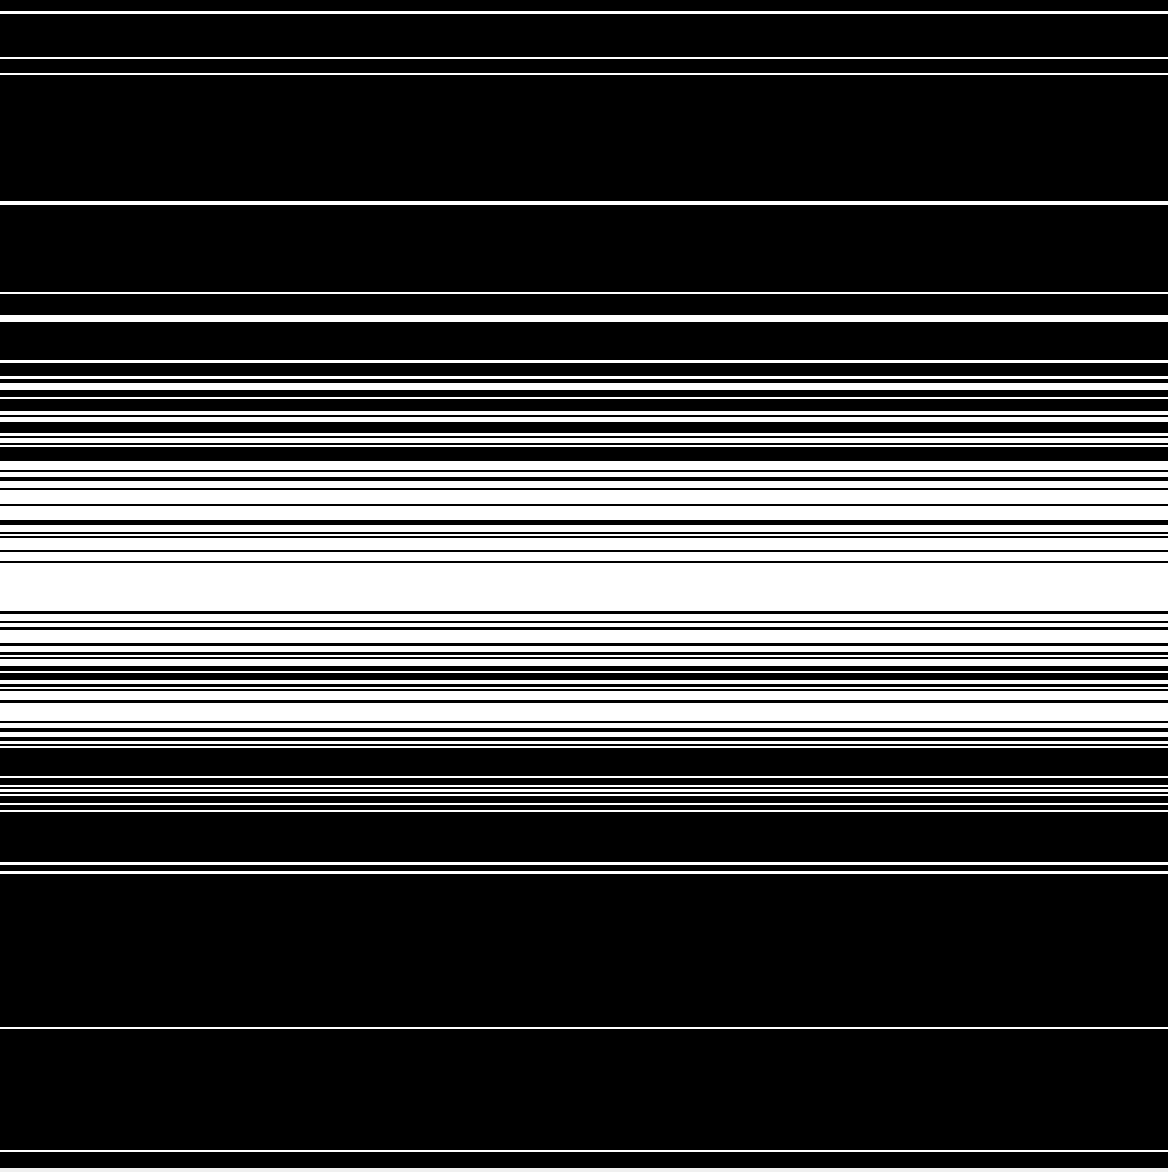
\includegraphics[width=2.5in]{img/intro/cartesian.png}
}
\subfigure[径向采样]{
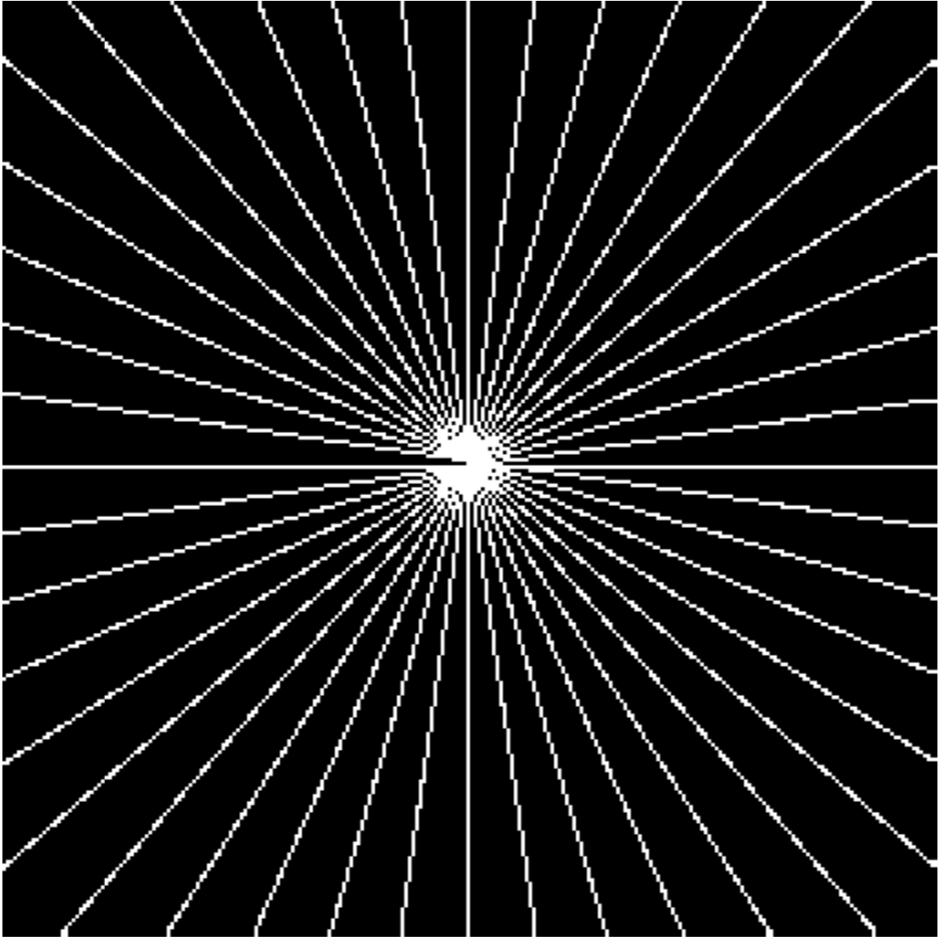
\includegraphics[width=2.5in]{img/intro/radial.png}
}

\subfigure[螺旋采样]{
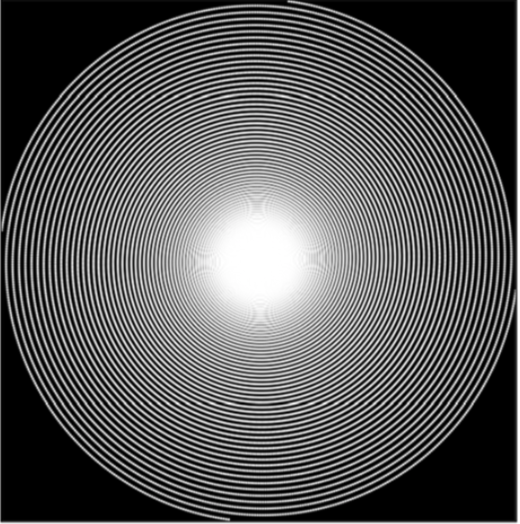
\includegraphics[width=2.5in]{img/intro/spiral.png}
}
\subfigure[变化密度采样]{
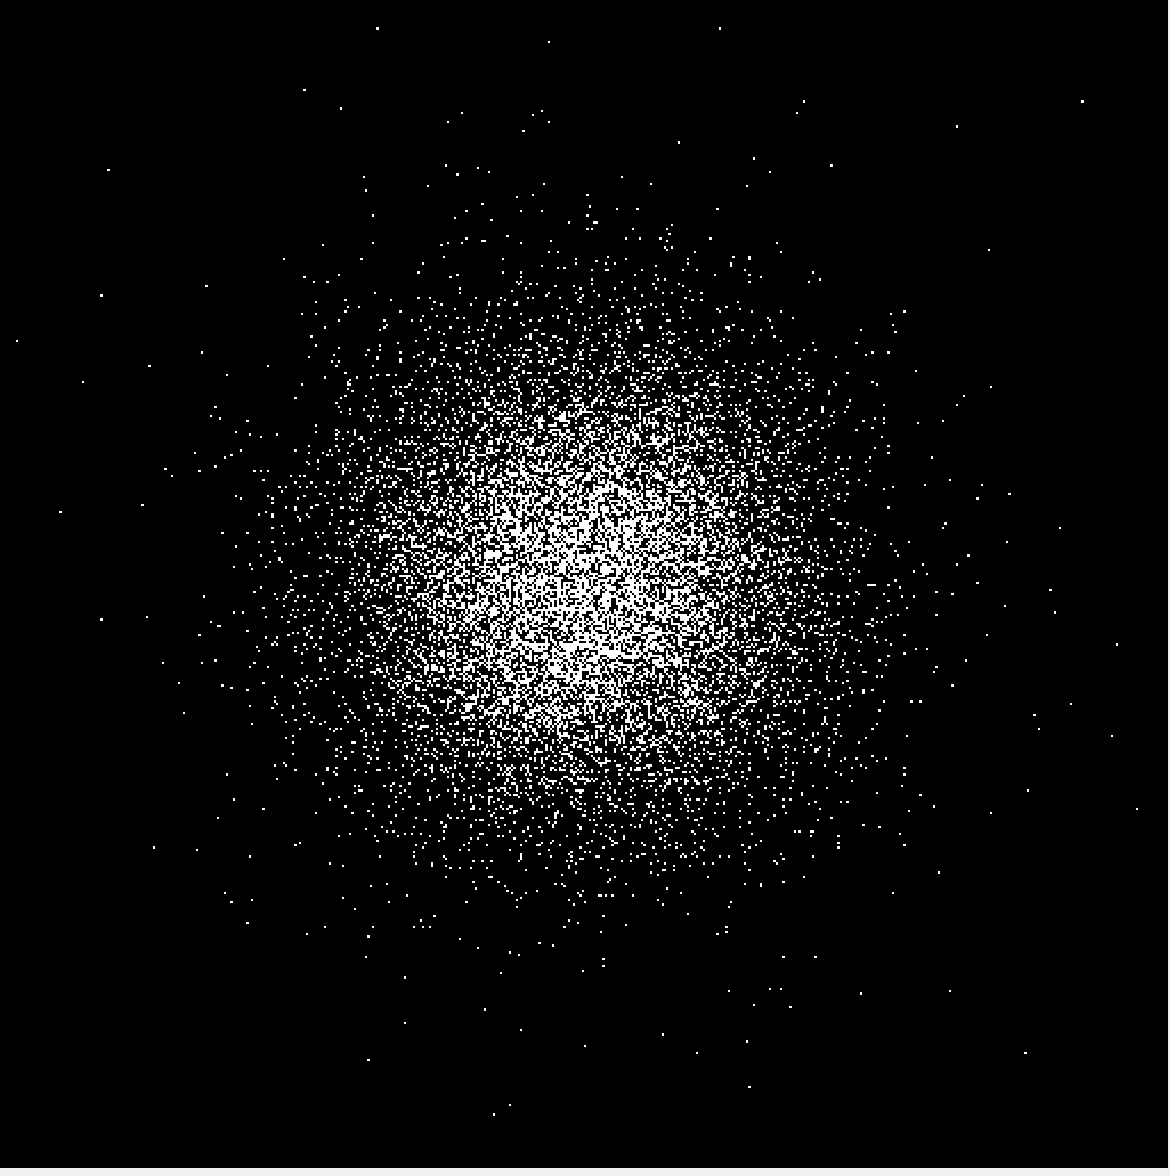
\includegraphics[width=2.5in]{img/intro/vd.png}
}
\centering
\caption{MRI中常用的采样模式}
\label{fig:mask}
\end{figure}

如何设计压缩感知MR重建的采样模式一直是研究人员所关心的话题,也决定着重建图像质量的好坏和重建算法的速度。设计的思路之一是将以上四种采样模式进行组合。比如,对于二维MR成像,伪径向采样\cite{Sajan2011Accelerated}(pseudo radial sampling)也是常见的采样模式,如图\ref{fig:maskdynamic}所示。伪径向采样结合了Cartesian和径向采样的优点,其采样点均在Cartesian网格上,同时使得采样点尽量沿径向方向。这样既可以获得高的采样率,又简化了计算。对于动态MR成像或者三维MR成像,由于其冗余性体现在多个维度上,采样矩阵的设计有了更大的空间。文献\cite{smith2012}针对胸部DCE-MRI图像,结合了Cartesian采样和随机采样,如图\ref{fig:maskdynamic}(a)所示。具体来说,在每一帧图像上使用Cartesian采样,并使得帧与帧之间采样有最大的正交性。文献\cite{Sajan2011Accelerated}中针对动态MR图像,结合了伪径向采样和随机采样,如图\ref{fig:maskdynamic}(b)所示。具体来说,在每一帧图像上均匀地选取一些伪径向采样线,并使得帧与帧之间的采样线随机转动一个角度以增加非相干性,即在空间上采用伪径向采样,在时间上采用随机采样,这也是动态MR采样模式的设计思路之一。文献\cite{holland2013compressed}针对fMRI图像,采用了变化密度螺旋采样模式。具体来说,这种采样方式使得k-space中心区域可以达到Nyquist采样率,而k-space的外围则是下采样,从而增加了采样的非相干性。除了fMRI,变化密度螺旋采样也被应用在心脏电影成像\cite{kressler2007three}、扩散张量成像\cite{karampinos2009high}、心脏血管造影成像\cite{santos2006single}中。

\begin{figure}[htbp]
\centering
\subfigure[动态Cartesian采样]{
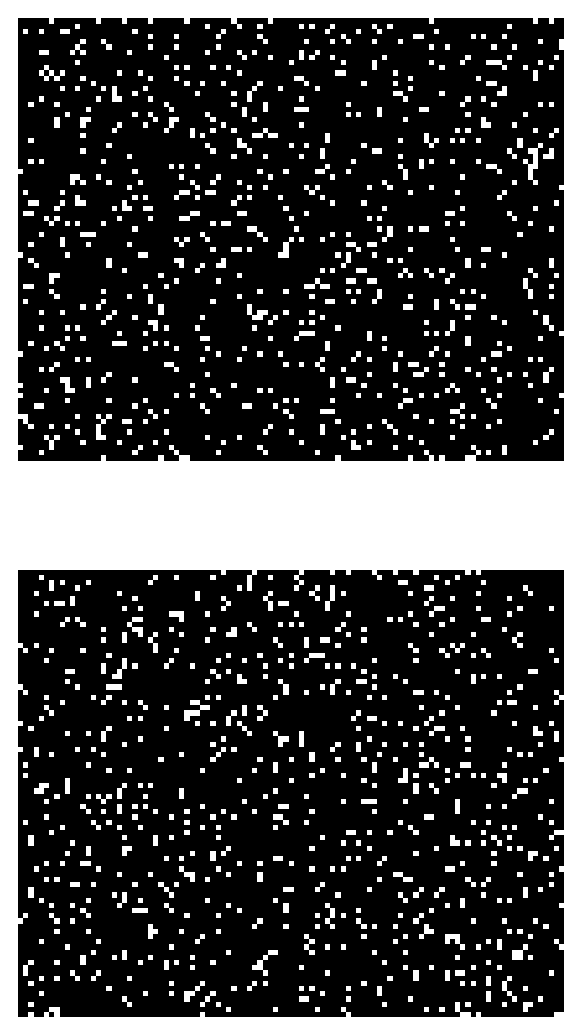
\includegraphics[width=1.645in]{img/intro/dynamic.eps}
}
\subfigure[动态伪径向采样(一帧)]{
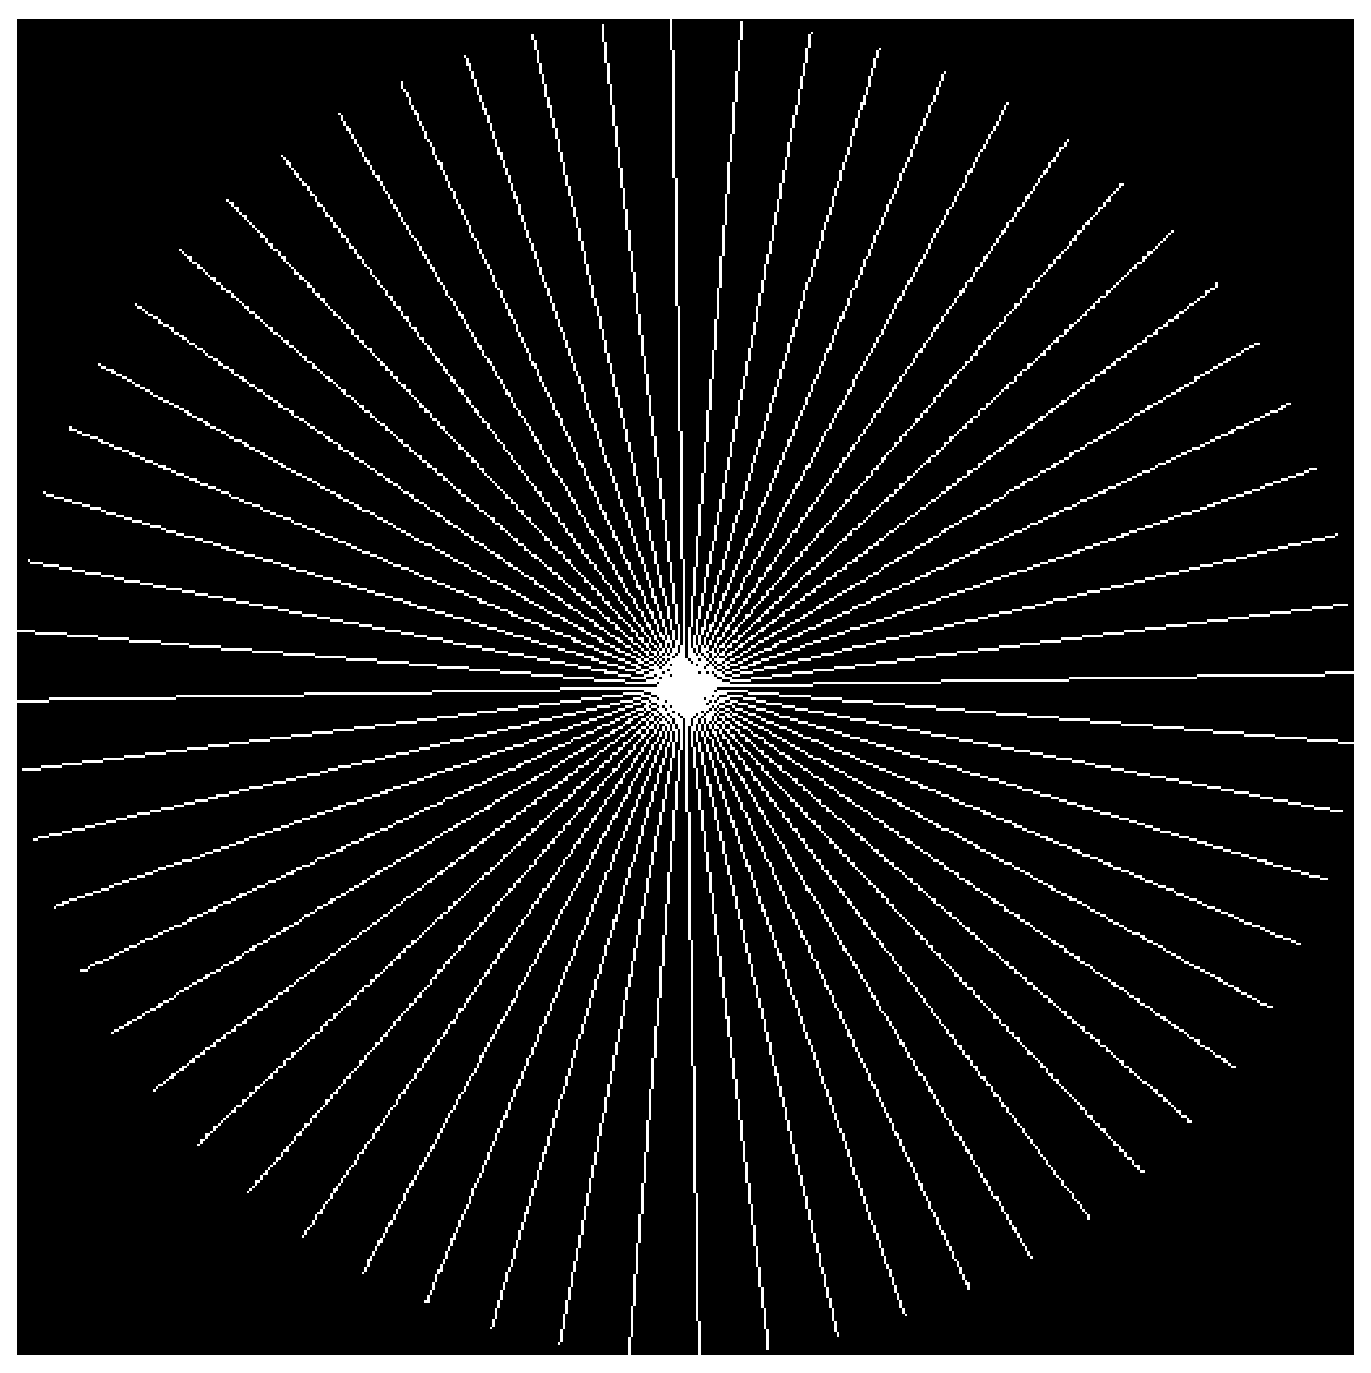
\includegraphics[width=3in]{img/intro/pradial.eps}
}
\caption{动态MRI中常用的采样模式。}
\label{fig:maskdynamic}
\end{figure}

综上所述,压缩感知MR重建的采样矩阵既需要满足非相干性,也需要考虑MR的物理限制。对于二维MR成像,主要的采样模式有Cartesian采样、径向采样和螺旋采样;而对于动态MR成像和三维MR成像,冗余性体现在多个维度上,采样矩阵的设计有着更多的自由度。一般的思路是在根据不同的问题,在不同的维度上选择不同的采样模式。

\subsection{MR图像的重建模型}
\label{sec:models}
在这一小节,我们介绍压缩感知MR成像的经典模型,更详细的综述请参考文献\cite{ravishankar2019image,ye2019compressed}。我们知道,MR的数据获取发生在k-space中,即Fourier域中。则MR成像的采样矩阵$A\in \mathbb{C}^{M\times N}$,$M<<N$可以写成
\begin{equation}
	A=\mathcal{MF}
\end{equation}
其中$\mathcal{F}$为Fourier变换,$\mathcal{M}$为采样模式。则MR成像的数据采集过程可以建模为:
\begin{equation}
	b=Ax+\epsilon.
\end{equation}
压缩感知理论旨在寻找最稀疏的解,于是MR成像的压缩感知模型为:
\begin{equation}
\begin{aligned}
	\hat{x}&=\argmin_x \|\mathcal{S}x\|_1,\\
	&s.t.\quad \|Ax-b\|_2^2 \leq \epsilon.
	\label{equ:sampling}
\end{aligned}
\end{equation}
这里$x\in \mathbb{C}^N$为待重建图像,$b\in\mathbb{C}^M$为测量得到的k-space数据。将问题(\ref{equ:sampling})写成无约束优化问题为:
\begin{equation}
	\hat{x}=\argmin_x \|Ax-b\|^2_2+\alpha\|\mathcal{S}x\|_1.
\end{equation}
目前稀疏变换$\mathcal{S}$的选取方法有很多。根据稀疏变换选取方式的不同,可以把模型分为两大类,即基于模型(model-based)和基于数据(data-based)。

最早将压缩感知应用MR成像的是Lustig\cite{lustig2006}。在文章中,作者研究了适用于MR的稀疏表示,讨论了不同采样模式非相干性的大小,并提出了基于小波变换和全变分的MR重建模型:
\begin{equation}
	\min_x\frac{1}{2}||Ax-b||^2_2+\alpha ||\mathcal{W}x||_1+\beta \|x\|_\mathrm{TV}.
	\label{equ:wandtv}
\end{equation}
其中$\mathcal{W}$为小波变换,$\|\cdot\|_\mathrm{TV}$定义为:
$$\|\cdot\|_\mathrm{TV} = \|\nabla\cdot\|_1,$$
而
$$|\nabla\cdot|_1=\sqrt{(\nabla_x \cdot)^2+(\nabla_y \cdot)^2}.$$
其中$\nabla_x$和$\nabla_y$分别为$x$和$y$方向上的梯度算子。

Lustig使用了伪径向采样方式,并且利用共轭梯度下降法来求解模型(\ref{equ:wandtv})。由与共轭梯度法运行速度慢,针对这个模型,很多文章在重建算法上做了改进。Ma等在2008年提出了一种算子分裂算法TVCMRI\cite{tvcmri},2009年Yang等提出了基于交替方法的重建方法RecRF\cite{Yang2010A}。这两种方法都加快了算法的收敛速度,提高了重建图像的信噪比。2011年Huang\cite{Huang2011Efficient}等提出了结合算子分裂和变量分裂的算法FCSA(fast composite shrinkage algorithm),解决了FISTA只能处理一个稀疏项的瓶颈。

由于模型(\ref{equ:wandtv})中含有TV正则项,重建得到的图像往往会产生所谓的阶梯效应。为了解决这个问题,Bredies等\cite{bredies2010total}提出了利用高阶梯度项来刻画图像的TGV(total generalized variation)泛函,并将其应用在图像去噪\cite{infimaltgv}和压缩感知\cite{tgv}中。在实际应用中,一般使用二阶TGV,即$\mathrm{TGV}_{\alpha}^2$,其定义为:
$$\mathrm{TGV}_\alpha^2(x)=\argmin_v \alpha_1\|\nabla x-v\|_1+\alpha_0\|\mathscr{E}(v)\|_1.$$
这里$\nabla \cdot=(\nabla_x \cdot, \nabla_y \cdot)$一阶有限差分算子,$v$属于离散复值向量场$V\in \mathbb{C}^{2N}$,$\mathscr{E}(v)=(\nabla v+\nabla v^T)/2$是二阶对称导数算子。关于TGV的详细概念和性质请参考第\ref{chap:tgvlr}章。于是基于TGV的压缩重建模型为:
\begin{equation}
	\min_x\frac{1}{2}||Ax-b||^2_2 + \mathrm{TGV}_{\alpha}^2(x).
	\label{equ:tgv1}
\end{equation}
模型(\ref{equ:tgv1})使用主对偶算法求解,有关模型求解的详细推导过程和收敛性分析请参考第\ref{chap:tgvlr}章。基于二阶TGV的压缩感知模型可以在保持图像边缘的同时有效地抑制阶梯效应,并且提高重建图像的信噪比。

模型(\ref{equ:tgv1})的小波变换使用的Haar小波变换\cite{stankovic2003haar},其计算简便。在此之后,很多文献将Haar小波推广到了小波家族中其他更加复杂的变换,即多尺度几何分析。Curvelet\cite{candes2000curvelets}和Contourlet\cite{do2005contourlet}是多尺度几何分析中最早被提出的方法,可以很好的稀疏化表示图像中的曲线,而传统的小波变换只能表示图像中的点状特征。Shearlet\cite{easley2008sparse}变换具有对高维几何结构稀疏表示的能力,对于卡通类图像的最优稀疏近似和Curvelet相同,并且可以表示图像中边缘类纹理。在压缩感知的模型中加入多尺度几何分析,可以更好地恢复出图像中的高维几何信息和纹理信心。比如文献\cite{qu2010combined,qu2010iterative}将模型(\ref{equ:wandtv})中的小波变换$\mathcal{W}$换成了Curvelet变换和Contourlet变换,得到了以下两个模型:
\begin{equation}
	\min_x\frac{1}{2}||Ax-b||^2_2+\alpha ||\mathcal{CU}x||_1+\beta \|x\|_\mathrm{TV}
\end{equation}
和
\begin{equation}
	\min_x\frac{1}{2}||Ax-b||^2_2+\alpha ||\mathcal{CO}x||_1+\beta \|x\|_\mathrm{TV}.
\end{equation}
其中$\mathcal{CU}$和$\mathcal{CO}$分别为Curvelet变换和Contourlet变换。实验表明,这两个模型可以很好地恢复出图像中曲线状的几何信息。Gao等\cite{infimaltgv}基于图像分解的思想,提出了利用了二阶TGV和Shearlet变换的变分模型:
\begin{equation}
	\begin{aligned}
		\min_{x_1,x_2}\frac{1}{2}\|A(x_1+x_2)-b\|^2_2+\mathrm{TGV}_{\alpha,\beta}(x_1)+\gamma\|\mathcal{SH}(x_2)\|_1.
	\end{aligned}
	\label{equ:shearlet}
\end{equation}
其中$\mathcal{SH}$为Shearlet变换,$x_1$和$x_2$分别代表图像的卡通部分和纹理部分。模型(\ref{equ:shearlet})可以应用在多种图像处理的任务中,如图像去噪、图像去糊、压缩感知重建等。当用于压缩感知重建时,模型(\ref{equ:shearlet})可以很好地恢复出图像的卡通部分和纹理部分。

除了利用小波变换和梯度信息,近些年有一些方法利用了结构化稀疏(structured sparsity)的概念。结构化稀疏是一般稀疏正则化方法的推广和延伸,其旨在选择特殊结构的稀疏性,比如图(graph/group)或者网络(network)。对于MR图像而言,其稀疏性往往具有某种特殊结构,而利用这种结构可以增加图像的稀疏性,从而降低测量所需的个数。寻找小波变换系数的结构是结构化稀疏常用的一类方法。Chen等提出了一个基于小波树稀疏的压缩感知模型WaTMRI\cite{tree,chen2014exploiting}:
\begin{equation}
	\min_x\frac{1}{2}||Ax-b||^2_2+\alpha \|x\|_\mathrm{TV} + \beta (||\mathcal{W}x||_1 + \sum_{o\in \mathscr{O}}||\mathcal{W}x_o||_2).
\end{equation}
其中$\mathscr{O}$表示所有母子系数组的集合,$o$为$\mathscr{O}$的一个组,$x_o$是属于母子系数组的所有数据。利用小波树进行压缩感知重建可以有效地消除边缘伪影。

结构化稀疏的另一大类方法是基于图像非局部(nonlocal)\cite{peyre2008non,lou2010image,gilboa2008nonlocal}信息的方法,并且已经被应用于MR成像模型中,其表现比一般的正则项要好。非局部的方法的基本思想是将有相似结构特征的图像块(patch)聚合在一起进行处理,这样可以更好地利用图像的冗余性。Mehmet等\cite{akccakaya2011low}基于非局部的思想提出了低维结构自学习和阈值算法(low-dimensional-structure self-learning and thresholding, LOST),主要利用了下采样图像中的结构信息。算法首先使用k-space中心低分辨率图像学习得到具有相似解剖结构的图像块,然后将这些图像块通过某种相似性聚类算法整合在一起,这样做可以有效地去除重建图像中的空间伪影。Liang等\cite{liang2011sensitivity}研究了非局部TV(NLTV)正则化在SENSE重建中的应用。NLTV范数定义如下:
$$\|x\|_{\mathrm{NLTV}}=\|\nabla^wx\|_{2,1},$$
其中$\|\cdot\|_{2,1}$是矩阵范数,即先对矩阵的每一列求$l_2$范数,再对所得结果求$l_1$范数。$\nabla^wx$是一个$N\times N$矩阵,表示加权非局部图像的梯度,其定义为:
$$\nabla^wx=[\nabla^w_{i,j}x],$$
其中$\nabla^w_{i,j}x$是像素点$i$与其非局部相邻像素点$j$之间的加权图像梯度:
$$\nabla^w_{i,j}x=\sqrt{w(i,j)}(x(i)-x(j)),$$
而$w(i,j)$是像素值$x(i)$与$x(j)$之间的图加权函数。将NLTV范数应用到MR重建中,其模型为:
\begin{equation}
	\hat{x}=\argmin_x \frac{1}{2}\|Ax-b\|^2_2+\alpha\|x\|_{\mathrm{NLTV}}.
\end{equation}
实验表明,NLTV模型可以很好地保持图像信息和细小的结构,并抑制噪声。Liu\cite{liu2017mri}等结合TV和NLTV,提出了基于图像块的JCTV模型:
\begin{equation}
\begin{aligned}
	\{\hat{x},\hat{z_i}\}=&\argmin_{x,z_i}\frac{1}{2}\|Ax-b\|_2^2+\sum_i\mu_{i,1}\|z_i\|_1\\
	&+\sum_i\mu_{i,2}\|z_i-\gamma_i\|_1,\\
	&s.t.\ z_i=\nabla\mathcal{P}_ix,
\end{aligned}
\end{equation}
其中$\mathcal{P}_i$算子表示从图像中取出图像块$x_i$,$z_i$是图像块在有限差分域的稀疏表示的系数,$\gamma_i$是真实图像的图像块块在有限差分与稀疏表示的系数,$\mu_{i,1}$和$\mu_{i,2}$是正则化参数。Qu等\cite{qu2014magnetic}提出了基于图像块的非局部算子(patch-based nonlocal operator, PANO)来对图像进行稀疏表示,并将其应用到了压缩感知成像中。同样令$\mathcal{P}_i$为块分解算子,图像的第$i$个块为$x_i$,则有$x_i=\mathcal{P}_ix$。将图像块按相似度分为$J$组,第$j$组的图像块记作$\mathcal{O}_{v_j}x_i$,其中$v_j$中为该组图像快的指标集。则非局部PANO算子定义为:
$$\mathcal{PANO}_j=\mathcal{S}\mathcal{O}_{v_j}\mathcal{P}_i.$$
将PANO算子应用到压缩感知的模型中:
\begin{equation}
	\hat{x}=\argmin_x \frac{1}{2}\|Ax-b\|_2^2 + \alpha\sum^J_{j=1}\|\mathcal{S}\mathcal{O}_{v_j}\mathcal{P}_ix\|_1.
\end{equation}
PANO算子可以稀疏化表示同一相似度的图像块,在MR重建中也取得了很好地效果。BM3D(Block Matching 3D)\cite{dabov2007image}也是通过将图像块分组的方法来处理图像非局部结构信息的模型,并被成功应用于图像去噪、去糊、超分辨率等任务中。Ender\cite{eksioglu2016decoupled}首次将BM3D模型应用到了MR重建中,并提出了模型BM3D-MRI:
\begin{equation}
	\hat{x}=\argmin_x \frac{1}{2}\|Ax-b\|^2_2+\alpha\|\Phi x\|_1,
\end{equation}
其中$\Phi\in\mathbb{C}^{K\times N}$为BM3D的分析框架,且$K>>N$,即框架$\Phi$是过完全的。文章使用了解耦算法来求解模型,并给出了算法收敛的条件。非局部BM3D-MRI是MRI重建模型的很有前景的应用。注意,利用结构化稀疏的模型中,有的也使用了基于数据的方法,比如PANO。因此称这些模型为部分基于模型更为准确。

到目前为止,我们讨论的模型都是基于模型的或者部分基于模型的。而压缩感知MR重建另一大类方法是通过学习的方法来学习图像的稀疏表示,即基于数据的(data-based)方法,或者称为盲压缩感知\cite{gleichman2011blind}(blind CS)。2011年,Ravishankar等提出了基于字典学习的压缩感知模型DL-MRI\cite{dlmri},这也是最早将学习的思想应用到MR重建中的模型。模型如下:
\begin{equation}
\begin{aligned}
	& \min_{x,\mathcal{D},Z}\ \frac{1}{2}||Ax-b||_2^2+\alpha\sum_{j=1}^N||\mathcal{P}_{j}x-\mathcal{D}z_j||_2^2,\\
	&s.t.\ ||z_j||_0\leq s, \|d_i\|_2=1, \forall i,j.
\end{aligned}
\end{equation}
其中$\mathcal{P}_j$算子表示从图像$x$中抽取一个小块$x_j$,即$x_j=\mathcal{P}_jx$;$\mathcal{D}\in \mathbb{C}^{K\times N}$是待学习字典,$K$为字典中原子的个数,$z_j$是小块$x_j$相对于字典$\mathcal{D}$的稀疏表示,即$z_j=\mathcal{D}x_j$。模型的求解分为两个子步骤,即字典学习和图像重建。模型通过交替方向法求解,在字典学习和图像重建之间迭代,直到收敛。其中字典学习的子步骤是在已知图像$x$的情况下,求解字典$\mathcal{D}$并计算图像$x$在该字典下的稀疏表示。模型为:
\begin{equation}
\begin{aligned}
	& \min_{\mathcal{D},Z}\ \sum_{j=1}^N||\mathcal{P}_{j}x-\mathcal{D}z_j||_2^2,\\
	&s.t.\ ||z_j||_0\leq s, \|d_i\|_2=1, \forall i,j.
\end{aligned}
\label{equ:dictlearning}
\end{equation}
字典学习的方法有很多\cite{ksvd,mairal2010online,rubinstein2009double},其中K-SVD\cite{ksvd}是字典学习中最经典的方法,DL-MRI中即使用了这种算法,最后重建的结果比基于模型的方法有了显著的提高。作者在文献\cite{ravishankar2017efficient}中对DL-MRI模型进行了修改,提出了SOUP-DIL(sum of outer products)图像重建模型。模型利用了总(aggregate)稀疏度的概念,并提出了如下正则项:
\begin{equation}
\begin{aligned}
	& \min_{\mathcal{D},Z}\ \sum_{j=1}^N||\mathcal{P}_{j}x-\mathcal{D}z_j||_2^2 + \alpha^2\|z_j\|_0,\\
	&s.t.\ \|d_i\|_2=1, \forall i.
\end{aligned}
\label{equ:soup}
\end{equation}
其中总稀疏度项为$\sum_{j=1}^N\|z_j\|_0$,权重为$\alpha^2$。实验表明,SOUP-DIL算法可以提高重建图像的质量。虽然利用字典学习的方式进行压缩感知的重建可以有效地学习到图像的特征,但字典学习过程中的超参数较多,比如图像块大小、字典大小等,并且没有理论上的方法来指导超参数的选择,只能凭借经验。这也是学习方法中普遍存在的问题。

由于字典学习的模型(\ref{equ:dictlearning})中使用了$l_0$范数,求解过程中会涉及到一个非凸的且NP难的优化问题\cite{bruckstein2009sparse},计算代价很大。Ravishankar针对这个问题提出了基于稀疏变换学习(sparsity-transform leaning,TL)的模型\cite{ravishankar2015efficient}。稀疏变换学习的方法十分有效,在很多面都有应用,并且可以保证算法的收敛性。具体来说,稀疏变换学习的正则项的定义为:
\begin{equation}
	\begin{aligned}
		\mathcal{R}(x)=&\min_{\mathcal{S},Z}\sum_{j=1}^N\|\mathcal{S}\mathcal{P}_jx-z_j\|^2_2,\\
		&+\alpha\mathcal{Q}(\mathcal{S}),\ s.t.\|Z\|_0\leq s, 
	\end{aligned}
\end{equation}
其中$\mathcal{S}\in \mathbb{C}^{n\times N}$是一个未知的变换,函数$\mathcal{Q}(\mathcal{S})$是关于这个变换的函数:
\begin{equation}
	\mathcal{Q}(\mathcal{S})=-\mathrm{log}|\mathrm{det}\mathcal{S}|+0.5\|\mathcal{S}\|^2_\mathrm{F}.
\end{equation}
于是基于稀疏变换学习的重建模型为:
\begin{equation}
	\begin{aligned}
		&\min_{\mathcal{S},Z}\frac{1}{2}\|Ax-b\|^2_2\sum_{j=1}^N\|\mathcal{S}\mathcal{P}_jx-z_j\|^2_2\\
		&+\alpha\mathcal{Q}(\mathcal{S}),\ s.t.\|Z\|_0\leq s.
	\end{aligned}
	\label{equ:slmri}
\end{equation}
模型(\ref{equ:slmri})的最重要的优势是更新$\mathcal{S}$的时候存在闭形式的解,因此也避免了字典学习更新中的繁琐计算。目前,基于稀疏变换学习的重建模型已经有了很多推广,比如STL-MRI\cite{ravishankar2015efficient}、UNITE-MRI\cite{ravishankar2016data}、FRIST-MRI\cite{wen2017frist}、STROLLR-MRI\cite{wen2018power}等。详细的算法流程及综述请参考\cite{wen2019transform}。

最近几年,由于深度学习\cite{lecun2015deep,schmidhuber2015deep}(deep learning)的兴起和火热,出现了很多利用深度神经网络进行压缩感知重建的方法,如\cite{jin2017deep,admmnet,wang2016accelerating,lee2018deep,han2018deep,zhu2018image,unetcs,varnet,gannet}等。这大类方法的主要思路是通过神经网络来学习图像的特征,来建立下采样数据和真实数据之间的联系。根据处理图像域的不同,基于深度学习的MR重建可以分为四类,如图\ref{fig:deepmri}所示。其中图\ref{fig:deepmri}(a)是图像域的深度学习。此类方法首先从下采样的k-space数据中得到有高度空间伪影的Zerofilled图像,然后训练神经网络学习这些空间伪影,即训练一个从图像域到图像域的神经网络。此类网络的代表有深度残差学习\cite{lee2018deep}和域适应的神经网络\cite{han2018deep},可以有效地去重建图像中的空间伪影。目前图像域的神经网络的发展趋势是寻找更复杂精妙的损失函数来克服平滑化的伪影。图\ref{fig:deepmri}(b)是混合域的神经网络,这类网络是利用压缩感知模型中的数据项来进行训练和推断,将求解模型的优化算法展开成一个神经网络。这类方法是最常用的基于深度网络的重建方法。LISTA\cite{gregor2010learning}是最早使用这个思想的网络,其将ISTA算法\cite{beck2009fast}展开成了神经网络,来学习权重和稀疏变换。VARnet\cite{varnet}将如下优化问题展开成网络:
\begin{equation}
	\hat{x}=\frac{1}{2}\|Ax-b\|_2^2+\alpha\mathcal{R}(x).
\end{equation}
这里正则项$\mathcal{R}(x)$表示为多通道卷积运算的和:
\begin{equation}
	\mathcal{R}(x)=\argmin_x\sum_{i=1}^J\langle \sigma_i(\mathcal{C}_ix),\textbf{1}\rangle,
\end{equation}
其中$\mathcal{C}_i$为第$i$个通道的卷积算子,$\sigma_i$为对应的激活函数。在VARnet中,需要通过网络学习卷积算子$\mathcal{C}_i$、激活函数$\sigma_i$和$\alpha$。ADMM-NET\cite{admmnet}将ADMM算法的迭代步骤展开,并与深度神经网络的每一层一一对应。其他类似的网络有Primal-Dual\cite{adler2018learned}网络和投影梯度\cite{gupta2018cnn}网络。图\ref{fig:deepmri}(c)的方法直接通过深度神经网络学习频率域与图像域的映射,如AUTOMAP\cite{zhu2018image}。这种方法需要在卷基层后接上全连接层,因此对内存和存储的要求很高。最后一类是成像域(频率域)的神经网络,如图\ref{fig:deepmri}(d)所示。这类方法直接通过神经网络学习频率域的差值并进行去噪操作,应用到MR重建中的网络有\cite{han2019k,lee2019k}等。基于深度学习的重建算法本质上是通过神经网络学习图像的特征,如稀疏变换、空间伪影或者噪声等,其重建的效果也比一般基于模型的方法更好。但是,深度神经网络的超参数很多,比如卷积核的大小、激活函数的选择等,并且深度学习目前没有建立普遍适用的理论基础,这也是其最被诟病的一点。
\begin{figure}[htbp]
\centering
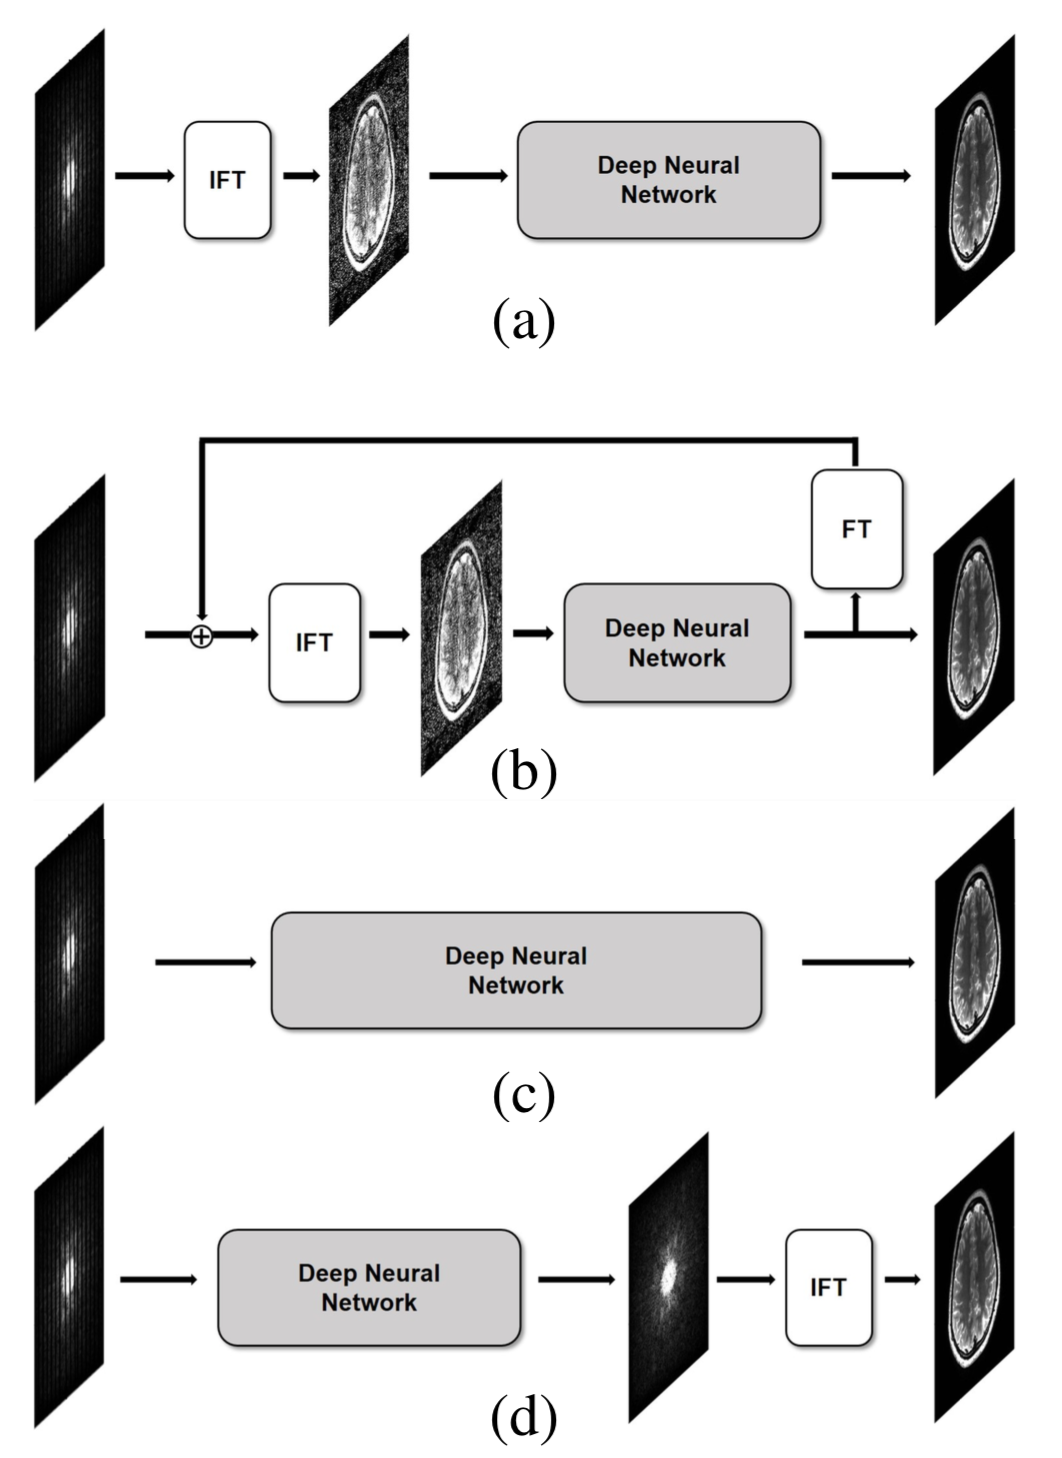
\includegraphics[width=0.9\textwidth]{img/intro/deepmri.png}
\caption{基于深度学习的MR重建。此图来自文献\cite{ye2019compressed}。}
\label{fig:deepmri}
\end{figure}

综上所述,基于压缩感知的MR重建模型分为基于模型和基于数据两大类。其中基于模型的方法是根据图像的先验特征选择或者构造稀疏项,比如TV、TGV、小波变换、多尺度分析、非局部算子等。这类方法一般有着坚实的数学理论做支撑,算法的收敛性也有保证。基于数据的方法是从数据中学习图像的稀疏项,主要有字典学习、稀疏变换学习、深度学习等。这类模型的重建结果一般比基于模型的方法要好,但是其超参数通常很多,而且计算量大。因此,在实际应用中,需要根据实际问题选择合适的模型。

\subsection{动态MR图像的重建模型}
\label{sec:dmri}
由于本论文主要针对动态MR图像,在这一小节我们介绍动态MR的压缩感知模型。动态MRI在临床中应用广泛,如心脏电影成像、心脏灌注、磁共振动态对比增强, 功能磁共振成像等。正如第\ref{sec:sparsity}小节所述,动态MR数据不仅包含了图像的空间信息,也包含了组织随时间变化的信息。因此,动态MR图像的冗余性不仅体现在空间方向上,也体现在时间方向上。设计动态MR图像的压缩感知模型的思路是利用好这两个方向上,尤其是时间方向上的冗余性。

为了与二维MR图像区分,我们记动态MR图像为$X\in \mathbb{C}^{N_1\times N_2\times d}$, 其中$d$为时间方向的维度。于是动态MR压缩感知的模型为:
\begin{equation}
\begin{aligned}
	\hat{X}&=\argmin_X \|\mathcal{S}X\|_1,\\
	&s.t.\quad \|AX-B\|_\mathrm{F}^2 \leq \epsilon
\end{aligned}
\label{equ:dynamic}
\end{equation}
这里$\mathrm{F}$为矩阵的Fobienus范数,$B$为下采样数据矩阵,我们称之为kt-space数据。将问题(\ref{equ:dynamic})写成无约束优化问题:
\begin{equation}
	\hat{X}=\argmin_X \frac{1}{2}\|AX-B\|_\mathrm{F}^2+\alpha\|\mathcal{S}X\|_1.
\label{equ:dunconstraint}
\end{equation}

最早将压缩感知应用到动态MR图像上的模型是k-t SPARSE\cite{lustig2006}。模型使用了空间和时间方向的稀疏性,其中空间方向上的稀疏变换为小波变换,而时间方向上使用了一维Fourier变换。其模型如下:
\begin{equation}
	\min_X\frac{1}{2}||AX-B||_\mathrm{F}^2 + \alpha||\mathcal{W}X||_1 + \beta||\mathcal{F}_tX||_1.
\end{equation}
其中$\mathcal{F}_t$为时间方向上的一维Fourier变换。模型采用了Cartesian随机采样,使用共轭梯度法求解。由于Fourier变换具有周期性,这个模型在心脏电影成像中的重建结果很好,但在其他动态MR图像中的应用有限。

Jung等提出了基于经典k-t BLAST/SENSE\cite{Jeffrey2003k}的改进算法k-t FOCUSS\cite{focuss,jung2007improved},并且k-t FOCUSS最重要的贡献之一是揭示了动态MR压缩感知模型和传统的k-t方法的差别不大,而且可以通过简单修改k-t BLAST/SENSE来得到。k-t FOUCSS的模型为:
\begin{equation}
\begin{aligned}
		\min_X &||X||_1,\\ 
		s.t.&\quad ||A\mathcal{F}_tX-B||_\mathrm{F}^2\leq \epsilon.
\end{aligned}
\label{equ:focuss}
\end{equation}
%注意这里与一般的模型不同,$X$属于Fourier域,即x-f space。
k-t FOCUSS主要的想法是利用残差编码和预测。具体来说,我们将$X$分解为预测信号$X_0$和残差信号$\Delta X$:
\begin{equation*}
	X=X_0+\Delta X.
\end{equation*}
因此模型(\ref{equ:focuss})变为:
\begin{equation}
\begin{aligned}
		\min_X &||\Delta X||_1.\\ 
		s.t.&\quad ||A\mathcal{F}_tX_0+A\mathcal{F}_t\Delta X-B||_\mathrm{F}^2\leq \epsilon.
\end{aligned}
\end{equation}
k-t FOCUSS的目标是预测图像$X_0$并且使残差图像$\Delta X$尽量稀疏。注意模型中只有时间方向的稀疏变换$\mathcal{F}_t$,而没有空间方向的稀疏变换。

Li等结合压缩感知、平行成像和黄金角度径向采样的想法,提出了iGRASP\cite{igrasp},模型如下:
\begin{equation}
	\min_X\frac{1}{2}||AX-B||_\mathrm{F}^2+\alpha||\nabla_t X||_1.
\end{equation}
这里黄金角度径向采样是指时间上相邻两条径向采样线的夹角是111.25$^{\circ}$,称为黄金角度。这样选择的好处是采样线可以覆盖整个kt-space并且在时间上保证非相干性。注意同k-t FOCUSS一样,iGrasp中只含有时间方向的稀疏项。

以上的几个模型在时间方向上使用了一维Fourier变换或者有限差分,而另一类方法是将矩阵的低秩性应用到动态MR图像重建模型中。低秩矩阵补全\cite{candes2009exact}(low-rank completion)将压缩感知的概念扩展到了矩阵,从而可以在低秩和非相干的条件下恢复出矩阵中丢失的信息。稀疏向量只有很少的非零元素,而类似的,低秩矩阵只有很少的非零特征值。低秩矩阵补全和压缩感知的结合可以进一步提高成像速度。这时,我们一般将$X$转化为一个时空矩阵,其中矩阵的每一列相当于动态MR图像的一帧,每一行相当于一个体素点。矩阵的结构如下所示:
\begin{equation}
X = 
\left[              
  \begin{array}{ccc}   
    X(p_1,t_1) & \cdots & X(p_1,t_{d})\\ 
    \vdots &\ddots & \vdots\\
    X(p_{N_1\times N_2},t_1) & \cdots & X(p_{N_1\times N_2},t_{d})\\  
  \end{array}
\right],                 
\end{equation}
其中$p_i,\ i=1,...,N_1\times N_2$为空间坐标,$t_i,\ i=1,...,d$。我们记为$X\in \mathbb{C}^{N_1N_2\times d}$。可以看出,由于时空上的相关性,$X$通常是一个低秩矩阵。图\ref{fig:lowrank}展示了一个动态图像的Casorati矩阵(a)。可以看出,矩阵的每一列只有很少的一部分有变化,大部分都是不变的,即这个矩阵的列秩很低。
\begin{figure}[htbp]
\centering
\subfigure[动态MR图像的Casorati矩阵]{
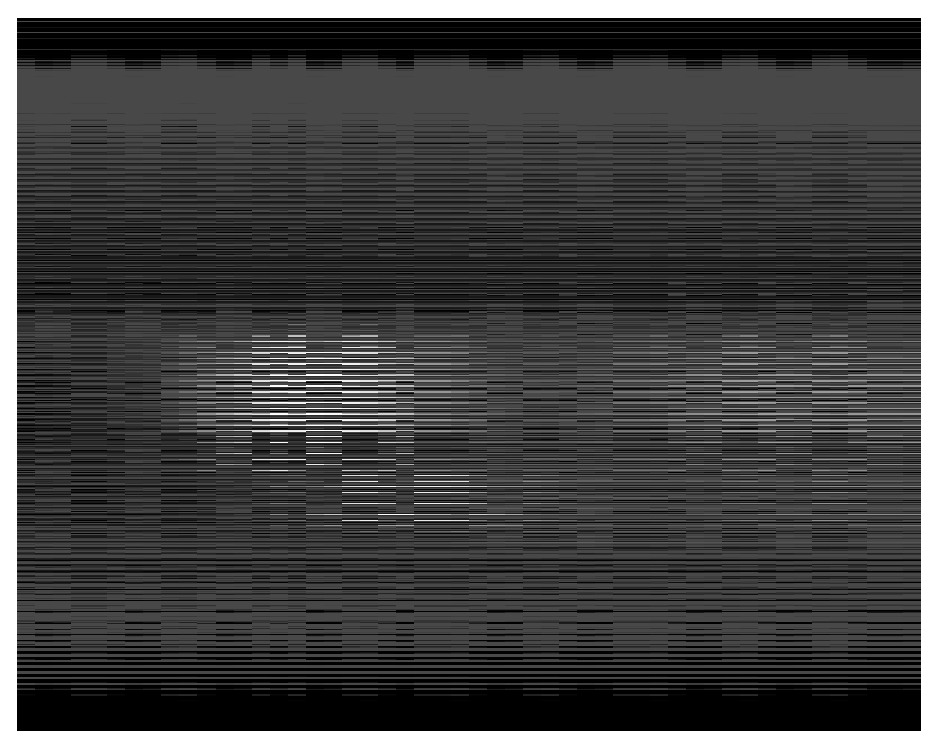
\includegraphics[width=2.5in]{img/intro/casorati.eps}
}
\subfigure[奇异值大小的变化]{
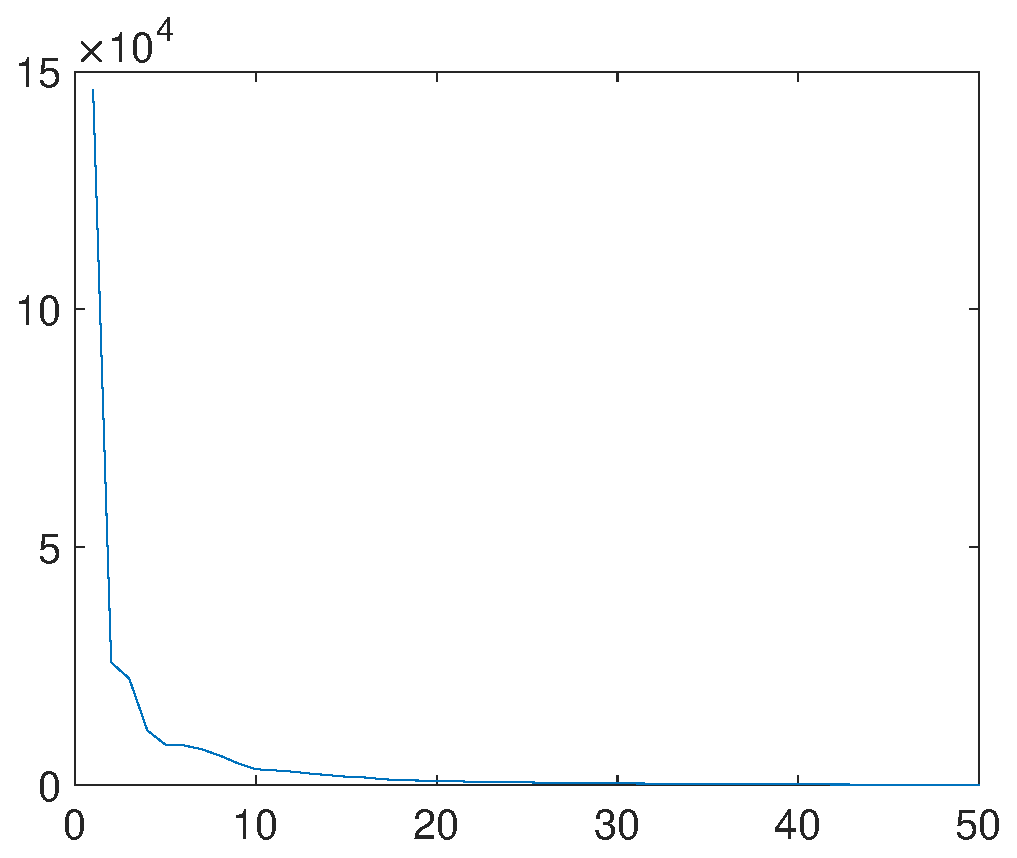
\includegraphics[width=2.5in]{img/intro/lowrank.eps}
}
\centering
\caption{动态图像的低秩性。}
\label{fig:lowrank}
\end{figure}

最早将矩阵的低秩性应用到MR重建中的模型为\cite{zhao2012image,Sajan2011Accelerated}。其中k-t SLR\cite{Sajan2011Accelerated}利用了三维TV和核范数,其模型如下:
\begin{equation}
	\min_X \frac{1}{2}||AX-B||^2_\mathrm{F}+\alpha\|X\|_{\mathrm{3DTV}}+\beta||X||_*.
\end{equation}
这里$\|\cdot\|_*$是矩阵的核范数,其定义为矩阵奇异值的和,即
$$\|X\|_*=\sum_i\sigma_i,$$
其中$\sigma_i$为$X$的奇异值。$\|X\|_{\mathrm{3DTV}}$定义为:
$$\|\cdot\|_\mathrm{3DTV}=\|\nabla_3\cdot\|_1,$$
而
$$|\nabla_3\cdot|=\sqrt{(\nabla_x \cdot)^2 + (\nabla_y \cdot)^2+(\nabla_t \cdot)^2},$$
其中$\nabla_x$,$\nabla_y$和$\nabla_t$分别为$x$,$y$和$t$方向上的梯度算子。核范数是矩阵的秩的凸松弛,被广泛应用于动态MR重建模型中。图\ref{fig:lowrank}(b)展示了一个Casorati矩阵奇异值大小的变化。可以看出,Casorati矩阵的奇异值只有很少一部分的值很大,大部分奇异值都接近于零,即其奇异值是$l_1$稀疏的。k-t SLR是第一个使用核范数作为时间稀疏项的模型,可以很好地稀疏化非周期性运动。k-t SLR采用伪径向采样,使用ADMM算法进行求解。模型在心脏体模数据和心脏电影成像的重建效果显著,但是重建算法的速度慢。

Otazo等基于矩阵低秩与稀疏分解的思想,提出了适用于动态MR图像的压缩感知重建模型L+S\cite{lpluss}。矩阵分解的目标是将矩阵$X$分解为低秩部分$L$与稀疏部分$S$:
\begin{equation}
	\min_{L,S}||L||_*+\lambda||S||_1, \quad s.t. \quad X=L+S.
\end{equation}
这个模型也被称为RPCA,Candès等\cite{rpca}建立了其数学基础,并指出,在特定的假设条件下,RPCA可以完美地恢复出低秩和稀疏部分,其中$L$的秩需要很低并且$S$需要有很高的稀疏度。图\ref{fig:l+s}展示了一个动态图像的低秩与稀疏分解的结果。可以看出,稀疏部分比原图像的稀疏度要高,而且图\ref{fig:l+s}(d)表明低秩部分的奇异值也比原图像要低。
\begin{figure}[htbp]
\centering
\subfigure[原图像]{
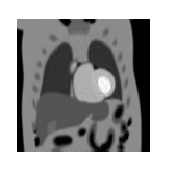
\includegraphics[width=2.5in]{img/intro/pincat.eps}
}
\subfigure[低秩部分]{
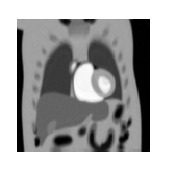
\includegraphics[width=2.5in]{img/intro/pincatl.eps}
}

\subfigure[稀疏部分]{
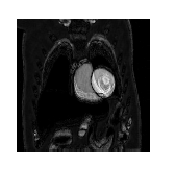
\includegraphics[width=2.5in]{img/intro/pincats.eps}
}
\subfigure[奇异值大小对比]{
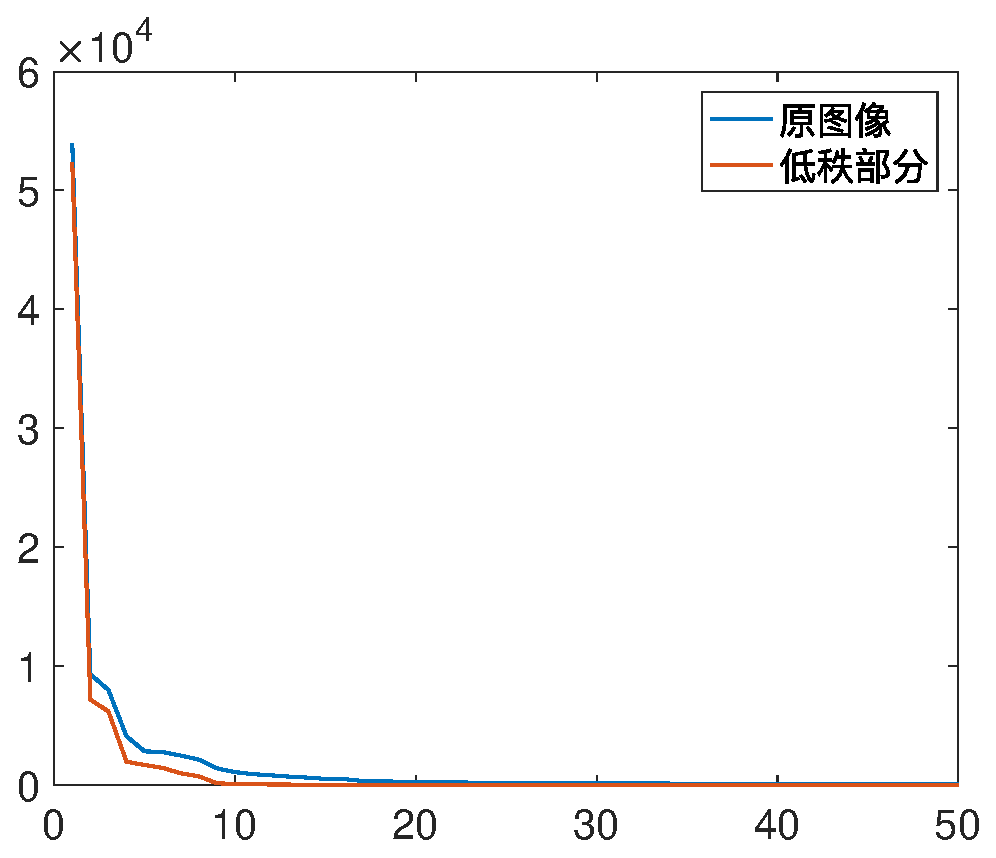
\includegraphics[width=2.5in]{img/intro/compare.eps}
}
\centering
\caption{动态图像的低秩稀疏分解(一帧)。}
\label{fig:l+s}
\end{figure}

将矩阵分解的想法应用在动态MR重建中,模型变为:
\begin{equation}
	\min_{L,S}||L||_*+\lambda||\mathcal{S}S||_1, \quad s.t. \quad A(L+S)=B,
\end{equation}
其中低秩部分$L$建模时间上高度相关的背景,稀疏部分$S$表征背景之上的动态信息。将模型转换为无约束问题:
\begin{equation}
	\min_{L,S}\frac{1}{2}||A(L+S)-B||_\mathrm{F}^2 + \alpha||L||_* + \beta||\mathcal{S}S||_1.
\end{equation}
文章中根据不同数据选择了不同的稀疏项$\mathcal{S}$。比如在心脏电影成像中,选择$\mathcal{S}$为时间方向的一维Fourier变换$\mathcal{F}_t$:
\begin{equation}
	\min_{L,S}\frac{1}{2}||A(L+S)-B||_\mathrm{F}^2 + \alpha||L||_* + \beta||\mathcal{F}_tS||_1.
\end{equation}
文献\cite{tremoulheac}中也使用了$\mathcal{F}_t$作为时间方向上的稀疏项。在血管造影中,选择$\mathcal{S}$为单位矩阵(即没有稀疏变换):
\begin{equation}
	\min_{L,S}\frac{1}{2}||A(L+S)-B||_\mathrm{F}^2 + \alpha||L||_* + \beta||S||_1.
\end{equation}
在胸部DCE-MRI中,选择$\mathcal{S}$为时间方向上的差分算子$\nabla_t$:
\begin{equation}
	\min_{L,S}\frac{1}{2}||A(L+S)-B||_\mathrm{F}^2 + \alpha||L||_* + \beta||\nabla_tS||_1.
\end{equation}
同样利用图像分解思想,Schloegl等 \cite{infimaltgv}提出了卷积下确界TGV泛函(infimal convolution TGV,ICTGV),其定义为:
\beq
\mathrm{ICTGV}_{\alpha, \beta}^2(X) = \inf_{X=X_1+X_2}\mathrm{TGV}_{\alpha_1}^2(X_1) + \beta\mathrm{TGV}_{\alpha_2}^2(X_2),
\eeq
相对应的重建模型为:
\beq
\min_{X}\frac{1}{2}||AX-B||_\mathrm{F}^2 + \mathrm{ICTGV}_{\alpha, \beta}^2(X).
\eeq
有关TGV的详细概念请参考第\ref{chap:tgvlr}章。

与结构化稀疏的概念类似,最近结构化低秩(structured low-rank)的概念也获得了广泛的关注,并且在MR成像上有着显著的应用前景。这类方法通过巧妙的构造Hankel结构化矩阵,将卷积运算转化为矩阵运算,然后通过极小化Hankel的秩构造并求解模型。这类方法的基本模型为:
\begin{equation}
	\begin{aligned}
		&\min_X\  \mathrm{rank}(\mathcal{H}(X)),\\
		& s.t. \ \mathscr{P}_\mathcal{O}(X)=\mathscr{P}_\mathcal{O}(B).
	\end{aligned}
\end{equation}
其中$\mathcal{H}$为Hankel结构化矩阵算子,$\mathscr{P}_\mathcal{O}$为指标集$\mathcal{O}$上的投影算子。注意这里的$X$同$B$一样,为kt-space数据,且目前结构化低秩的方法大多在kt-space中构造$\mathcal{H}$矩阵。主要的模型有SAKE\cite{shin2014calibrationless}、LORAKS\cite{haldar2013low}、ALOHA\cite{jin2016general,lee2016acceleration}、GIRAF\cite{ongie2016off}等,更详细的综述请参考文献\cite{ye2019compressed}。

除了以上基于模型的方法,基于学习的方法也被广泛地应用在动态MR成像中。Lingala\cite{lingala2013blind}提出了针对动态MR图像重建的盲压缩感知框架。对于一个动态MR图像$X\in \mathbb{C}^{N_1N_2\times d}$,盲压缩感知框架将其建模为两个矩阵的$\mathrm{U}\in \mathbb{C}^{N_1N_2\times K}$和$\mathrm{V}\in \mathbb{C}^{K\times d}$的乘积:
$$X=\mathrm{UV},$$
其中$K$为过完全字典中基函数的个数。这里$\mathrm{U}$为空间系数矩阵,其通常是稀疏的;而$\mathrm{V}$为包含时间基函数的字典。盲压缩感知模型即为从采样中估计$\mathrm{U}$和$\mathrm{V}$的过程:
\begin{equation}
\begin{aligned}
	\{\hat{\mathrm{U}},\hat{\mathrm{V}}\}=&\argmin_{\mathrm{U},\mathrm{V}}\frac{1}{2}\|A(\mathrm{UV})-B\|_\mathrm{F}^2+\alpha\|\mathrm{U}\|_1,\\
	&s.t.\ \|\mathrm{V}\|_\mathrm{F}^2\leq s.
\end{aligned}
\end{equation}
在自由呼吸心肌灌注MR图像上的实验表明,盲压缩感知模型对时空模糊更加鲁棒,并且更好地保持了精细的结构信息。Wang\cite{wang2013compressed}等针对动态心脏电影MR图像,提出了基于三维时空字典的模型:
\begin{equation}
	\begin{aligned}
		\min_{x,\mathcal{D},z_j}&\ \frac{1}{2}\|AX-B\|_\mathrm{F}^2+\frac{\alpha}{2}\sum_j\|\mathcal{P}_jx-\mathcal{D}z_j\|_2^2\\
		&+\beta\sum_j\|z_j\|_0+\gamma\|\mathcal{S}X\|_1.
	\end{aligned}
\end{equation}
这里与二维的情形不同,$\mathcal{P}_j$算子的作用是从图像$X$中提取时空图像块,且稀疏变换$\mathcal{S}$为3DTV算子。模型采用交替方向法求解,在字典学习和图像重建中进行迭代。类似的,Caballero等\cite{caballero2014dictionary}也基于心脏电影成像提出了时空字典学习模型。不同的是,Caballero模型中的稀疏变换为时间方向的梯度算子$\nabla_t$。Ravishankar等\cite{ravishankar2015efficient}基于图像分解的框架,并结合低秩的思想和字典学习的方法,提出了LASSI模型:
\begin{equation}
	\begin{aligned}
		&\min_{L,S,\mathcal{D},Z}\ \frac{1}{2}\|A(L+S)-B\|_\mathrm{F}^2+\alpha\|\mathcal{S}_1(L)\|_*\\
		&+\beta\{\sum_j\|\mathcal{R}_jS-\mathcal{D}z_i\|^2_2+\lambda^2\|Z\|_0\},\\
		& s.t. \ \|Z\|_\infty\leq a, \mathrm{rank}(\mathcal{S}_2(d_i))\leq r, \|d_i\|_2=1,\forall i.
	\end{aligned}
\end{equation}
数值试验表明,LASSI模型适用于多种动态图像,并且比一般的盲压缩感知方法的表现好。

近几年来,随着深度学习的兴起,深度神经网络也被广泛应用在了MR成像中。我们已经在第\ref{sec:models}中介绍了深度学习在二维MR图像重建中模型,但是其在动态MRI上的应用还处于起步阶段,模型不多。Schlemper等\cite{schlemper2017deep}首次将深度学习的思想应用在了动态MR图像重建中,提出了基于深度级联卷积神经网络(convolutional neural network,CNN),其模型为:
\begin{equation}
	\min_X \ \|X-f_{\mathrm{cnn}(X_z|\theta)}\|_\mathrm{F}^2+\alpha\|AX-B\|^2_\mathrm{F}.
	\label{equ:cnndmri}
\end{equation}
这里$f_{\mathrm{cnn}}$为CNN的向前映射,参数为$\theta$,其中包含了神经网络的权重,而$X_z$为Zerofilled图像。由于Zerofilled图像中包含着严重的空间伪影,CNN重建图像的过程可以看成是去除空间伪影的过程。该方法可以在高采样率下保持图像的解剖结构,且重建速度快。Qin等\cite{qin2018convolutional}提出了利用循环神经网络(convolutional recurrent neural network, CRNN)来重建动态MR图像。模型创新性地提出了双向卷积循环单元来学习图像在时空上的冗余性,在心脏图像重建中取得了很好地效果。Wang\cite{wang2018dimension}等在模型(\ref{equ:cnndmri})的基础上,提出了DIMENSION模型。模型同时利用了动态图像的k-space和空间先验信息,通过监督学习来训练网络。网络由两个主要部分构成,一部分为频率域网络,用于更新k-space;另一部分为空间域网络,用来提取图像中的高级特征。两部分网络通过Fourier变换进行连接。实验表明,DIMENSION可以提高重建图像质量,提高重建速度。Ke等\cite{ke2019crdn}提出了用于动态MR重建的级联残差密集网络CRDN。具体来说,网络利用了卷积层的多层级局部和非局部信息,并且使用了基于TV的增强边缘的损失函数。对比试验表明,CRDN可以在提高重建质量的基础上减少重建时间。

综上所述,动态MR图像的稀疏性不仅体现在空间上,也体现在时间上。而且,时间上稀疏项的选择是尤其重要的,可以很大程度上决定重建结果的好坏。目前,基于模型的方法既有传统的利用Fourier变换、TV的模型,也有利用图像的低秩性或结构低秩性和基于分解思想的方法。基于数据的方法相对较少,主要有训练时空字典的模型和搭建深度神经网络的方法。

\subsection{本节小结}
本节主要介绍了压缩感知在MR成像中的应用。我们首先讨论了MR图像的稀疏性和常见的采样模式,然后回顾了压缩感知MR成像的经典模型。最后由于本论文主要针对动态MR图像,我们也给出了动态MR图像压缩感知模型的综述。

\section{磁共振指纹的研究现状}
\label{sec:mrf}
磁共振指纹(magnetic resonance fingerprinting, MRF)是一种新的数据获取、后处理以及可视化的框架。与传统qMRI一次只能测量一个参数不同,MRF可以同时快速的量化多个组织参数,比如$T_1$,$T_2$,质子密度等,并且提高整个实验的信噪比和扫描效率。MRF主要由三个部分组成,分别为信号获取、预定义字典的生成和模式识别重建参数图。具体来说,首先针对特定的问题,选择一个合适的MR序列进行信号采集。然后利用MR成像的数学模型,生成一个信号演化的字典,字典中的每一个原子模拟了不同参数的组织在该MR序列下的信号演化,即包含着组织的参数信息。最后,使用模式识别算法将采集的信号与字典进行匹配,选择字典中最配的原子,其包含的参数信息即为该体素的参数。MRF的主要流程如图\ref{fig:mrf}所示。
\begin{figure}[htbp]
\centerline{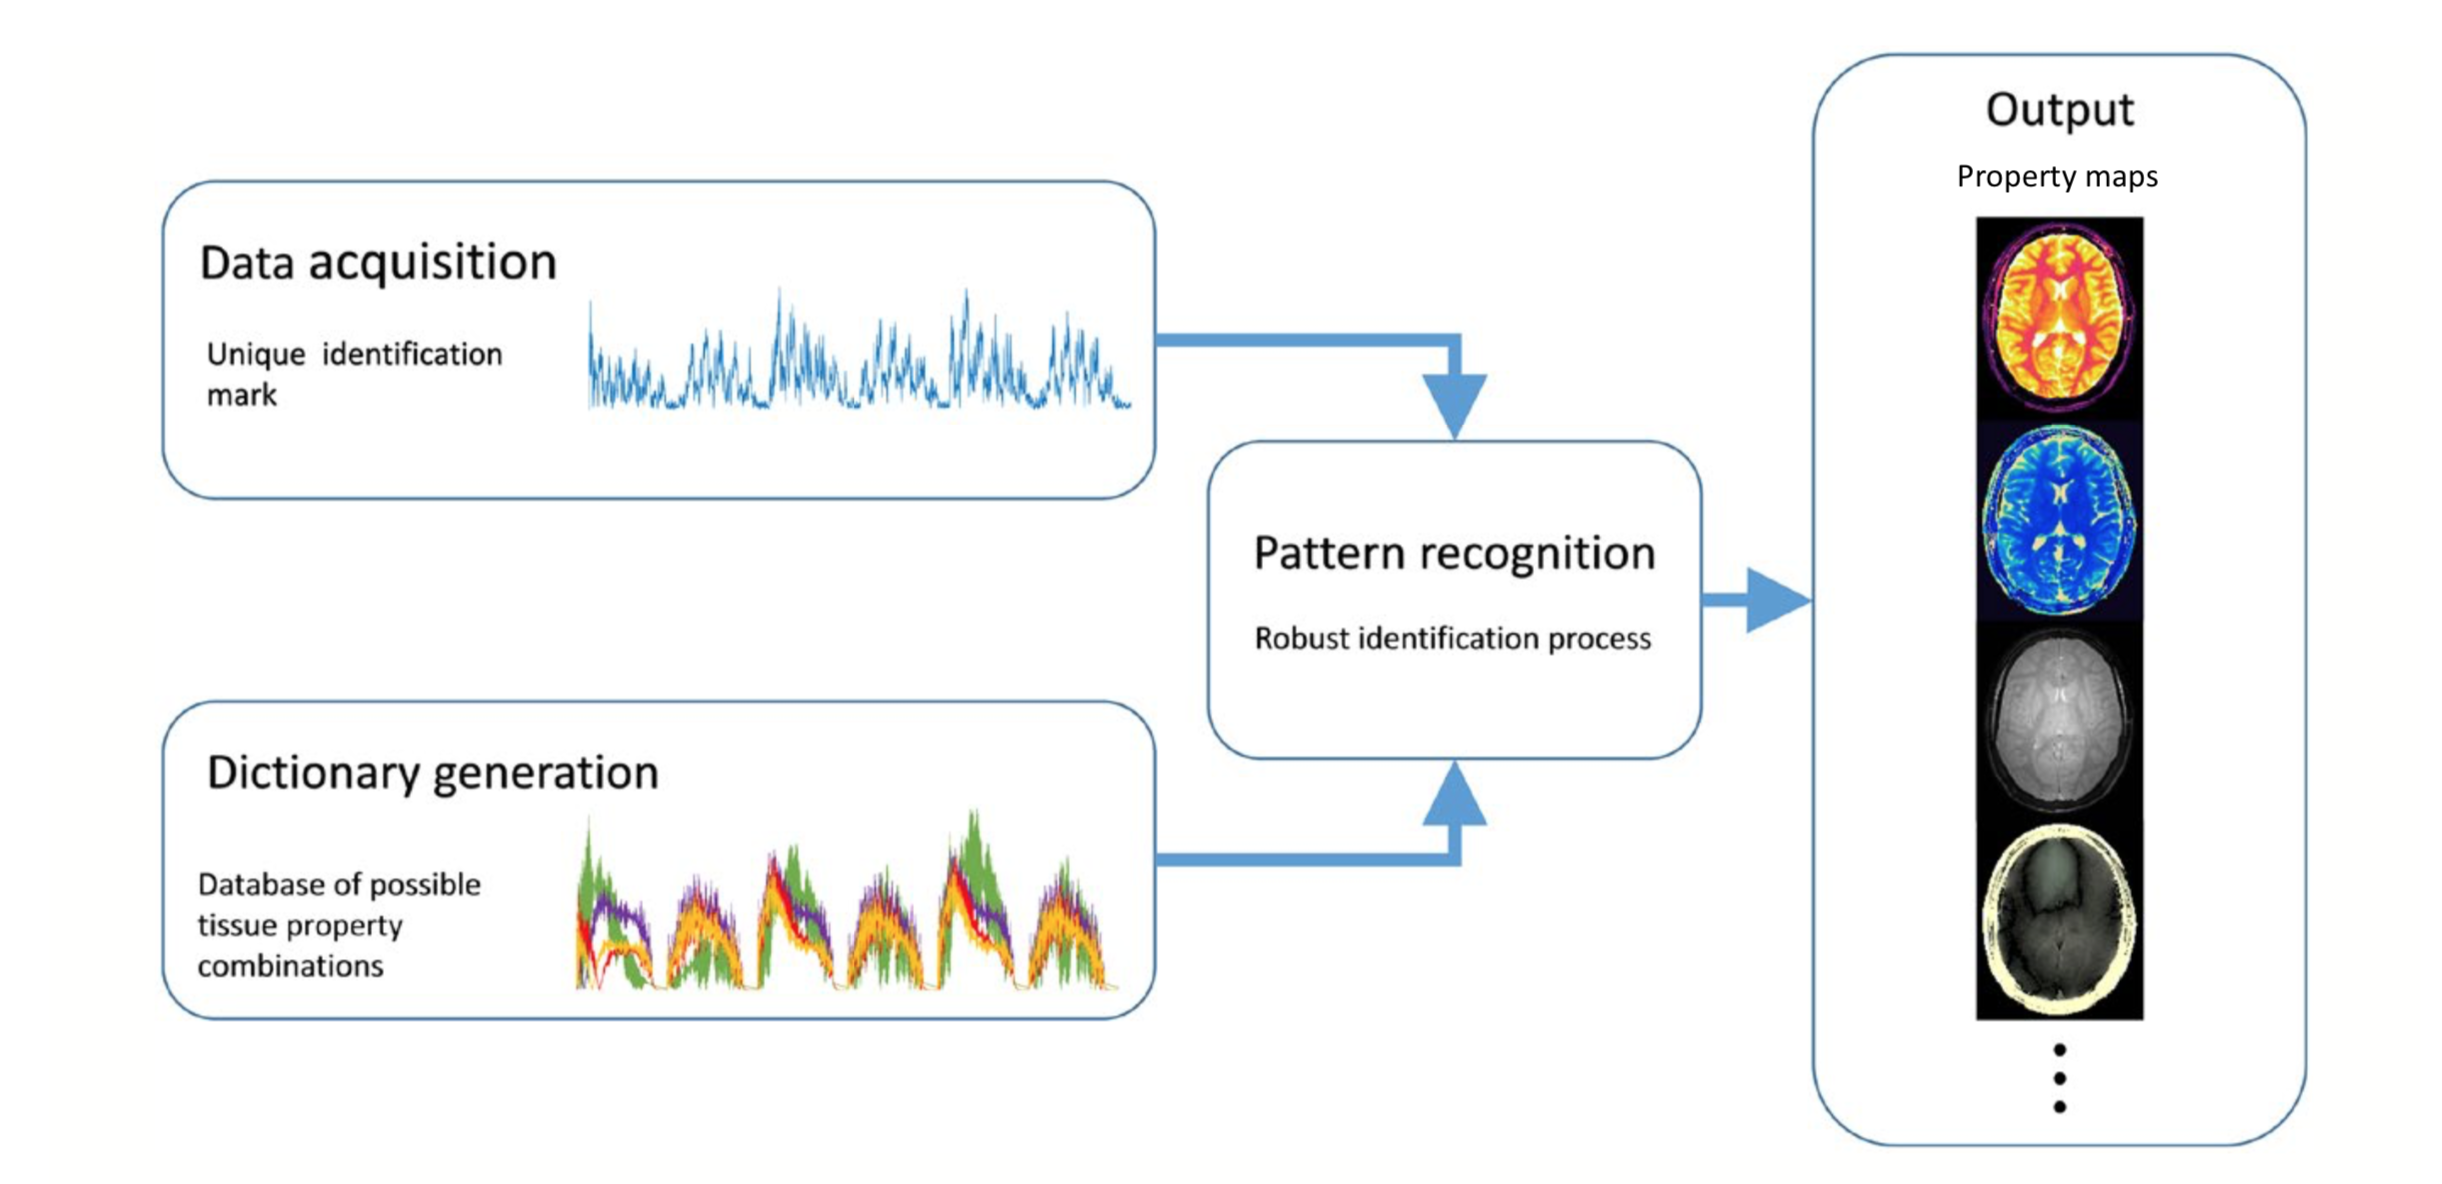
\includegraphics[width=1\textwidth]{img/intro/mrf.png}}
\caption{
MRF流程示意图。此图来自文献\cite{mrfreview}。
}
\label{fig:mrf}
\end{figure}

首先我们应该选取对所需参数敏感的MR序列对信号进行采样,并且序列的参数,如偏转角(flip angle),重复时间(repetition time, $T_\mathrm{R}$)需要随着时间随机变动,使得组织在MR序列中产生指纹状的信号演化。其次,字典中包含着不同参数的组织在该MR序列中的模拟演化。最后,模式识别算法用来比较每个像素指纹和字典中原子的匹配度,重建参数图。

\subsection{信号获取}
信号获取是MRF的第一步,我们首先需要根据具体问题,选择合适的MR序列进行信号采集。关于MR成像以及序列请参考第\ref{chap:pre}章。MR序列的选取需要满足以下三个方面。第一,选取的MR序列需要对我们所研究的参数敏感,如$T_1$,$T_2$等。第二,在数据采集过程中,采集参数如偏转角,重复时间等需要连续随机变化。第三,每隔$T_\mathrm{R}$时刻,使用伪随机下采样进行信号采集。图\ref{fig:fa}展示了偏转角(a)和重复时间(b)随时间变化的例子。这样做的目的是使不同参数的组织可以产生独特的信号演化,我们称之为指纹,即每个指纹中包含着不同组织的参数信息,以便在后面进行参数图重建。图\ref{fig:mrfimg}是某一$T_\mathrm{R}$时刻的体模和活体人脑的指纹图像。可以看出由于高度的下采样,图像中存在着感强烈的伪影。MRF重建的目标即是从指纹图像中重建出参数图。

\begin{figure}[htbp]
\centering
\subfigure[偏转角随时间的变化]{
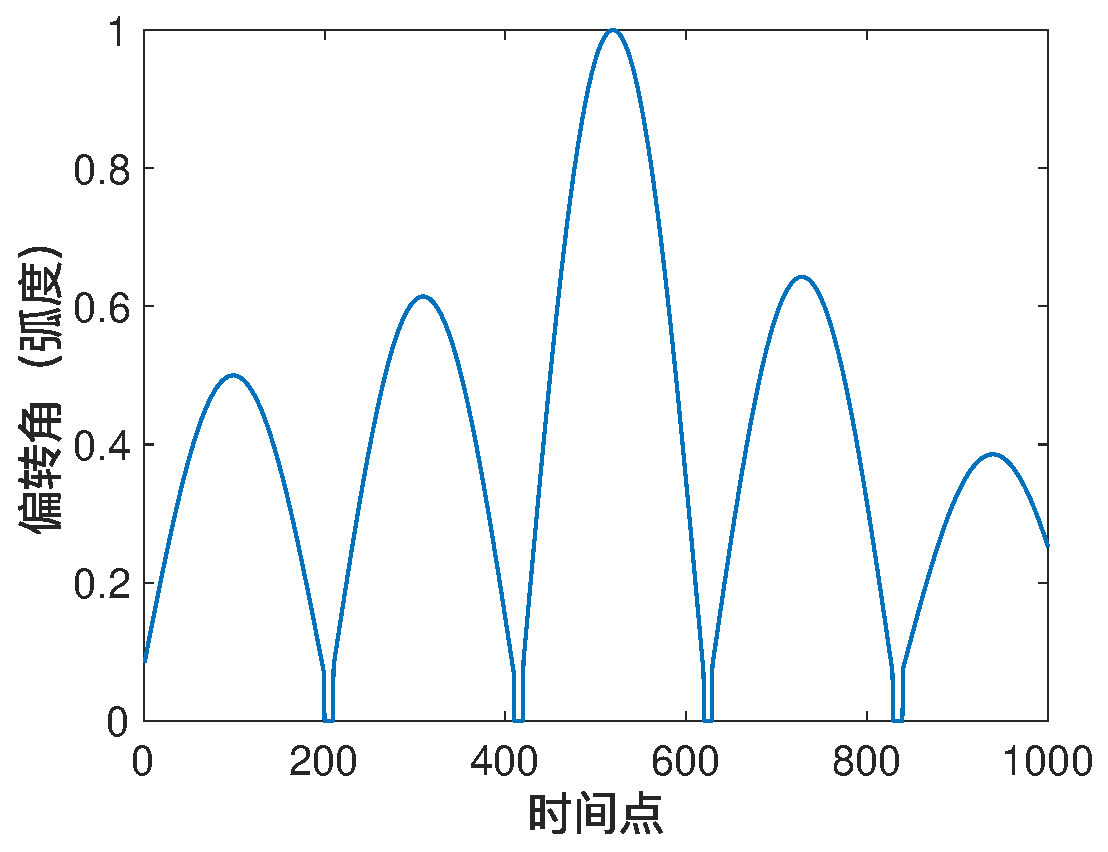
\includegraphics[width=3in]{img/intro/fa.eps}
}
\subfigure[重复时间随时间的变化]{
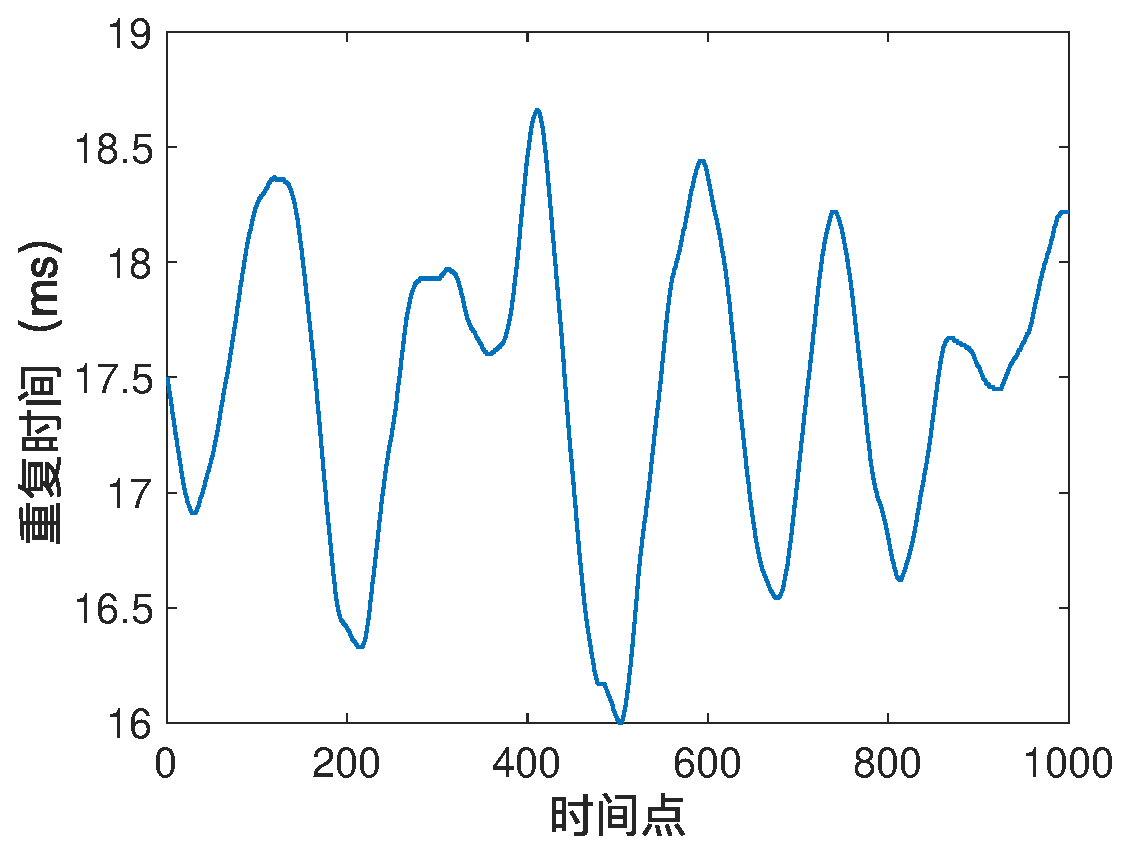
\includegraphics[width=3in]{img/intro/tr.eps}
}
\centering
\caption{偏转角(a)和重复时间(b)随时间的变化。}
\label{fig:fa}
\end{figure}

\begin{figure}[htbp]
\centering
\subfigure[体模指纹图像]{
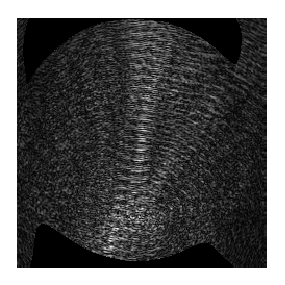
\includegraphics[width=2.5in]{img/intro/phantom.eps}
}
\subfigure[活体人脑指纹图像]{
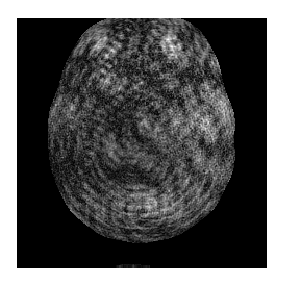
\includegraphics[width=2.5in]{img/intro/brain.eps}
}
\centering
\caption{指纹图像举例(某一时间点)。}
\label{fig:mrfimg}
\end{figure}

目前常用的MRF序列主要有两种。Ma\cite{mrf}在MRF的第一篇文章中使用了平衡稳态自由进动序列(balanced steady state free precession, bSSFP\cite{ussfp}),因为目前对bSSFP序列的研究最充分。bSSFP对$T_1$,$T_2$和$B_0$敏感,并且具有高信噪比、高扫描效率的性质。对于MRF来说,bSSFP是一个适合的序列。另一种常用的序列为FISP序列,或者称为非平衡稳态自由进动序列(unbalanced steady state free precession, uSSFP)。这个序列的特点是在每个$T_\mathrm{R}$结束之前,加上了一个非平衡的梯度场。Jiang\cite{jiang}等首先将uSSFP序列应用到了MRF上uSSFP序列有助于消除带状伪影,但是其只对$T_1$和$T_2$敏感,对$B_0$不敏感,因此不能获得$B_0$的参数图。其他种类序列的应用请参考文献\cite{joint,quest}。

\subsection{字典生成}
MRF字典中包含了不同参数的组织在MR序列中的模拟信号演化,字典中的每一个原子都包含着一组组织参数。因此,MRF的精度取决于生成字典所用的模型的精度和字典的大小。如果字典过小,则会导致重建参数图结果不精确;如果字典过大,生成字典和之后的匹配算法所需的时间就会增多。因此,需要在字典大小和重建速度之间寻找平衡。一般来说,对于一个给定的MRF序列来说,字典只需要生成一次,并且在之后的应用中保持不变。需要指出的是,MRF的字典和字典学习中的字典是不同的。MRF中字典的原子是组织的时间演化曲线,字典学习中字典的原子是基于图像块的特征。

目前生成字典主要有两种数学模型。Ma在\cite{mrf}中使用了简单的Bloch方程来模拟bSSFP序列中射频场和时序对于单一等色子(isochromat)的影响。模型假设指纹中的每个体素都由单一等色子构成。Bloch方程也可以应用在uSSFP中,但是会消耗更多的时间。这是因为在uSSFP中,由于非平衡梯度场的存在,指纹中的每个体素都是多个等色子的平均。因此Bloch方程在处理uSSFP时的效率不高。

扩展相图(extended phase graph, EPG\cite{weigel})是模拟uSSFP的另一种常用的模型。图\ref{fig:atoms}展示了EPG模型生成字典中的原子。EPG将体素内的自旋系统中描述为离散的状态矩阵,可以有效地表示自旋系统在非平衡梯度场的影响下随时间的演化。EPG的具体细节请看第\ref{sec:epg} 小节。EPG的另一个好处是可以在原有模型的基础上,加上其他参数的影响,如$B_0$,$B_1^+$,磁化转移(magnetization transfer)等。因此EPG在MRF中有着广泛的应用。但是由于EPG模型需要计算和存储等色子的状态矩阵,EPG的运行速度通常比较慢。
\begin{figure}[htbp]
\centering
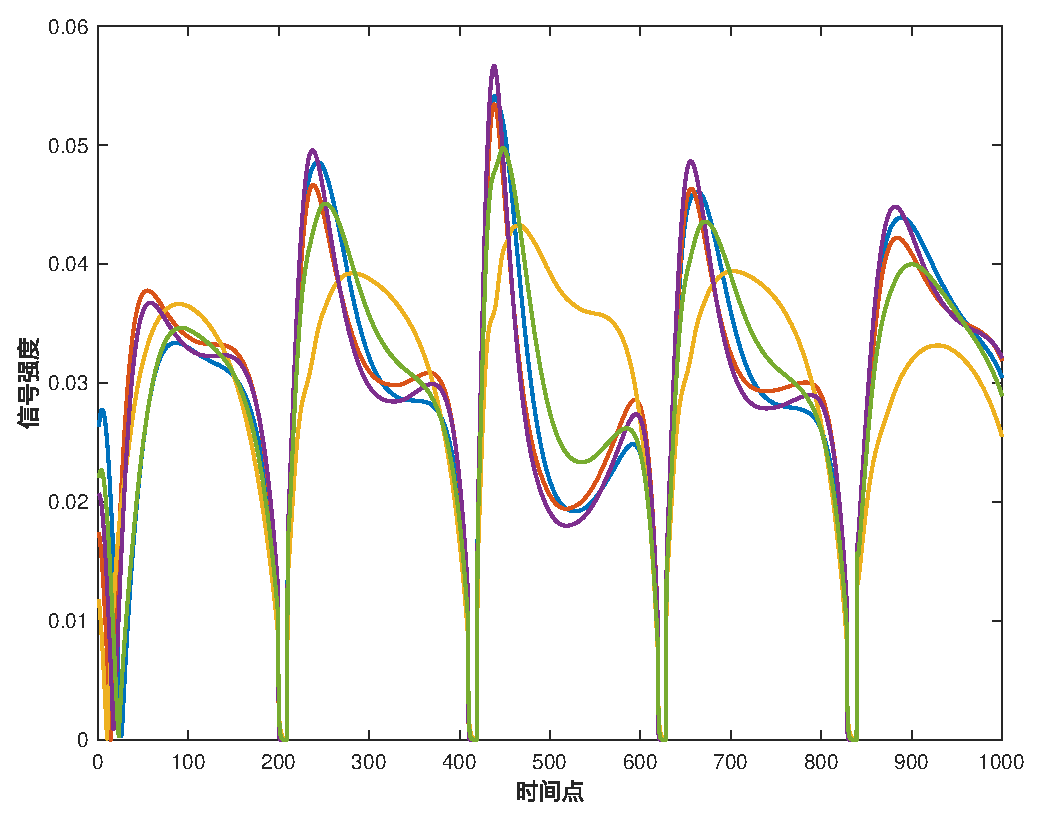
\includegraphics[width=0.8\textwidth]{img/intro/atoms.eps}
\caption{EPG模型生成的字典原子。}
\label{fig:atoms}
\end{figure}

\subsection{参数图重建}
MRF的最后一步是选择合适的匹配算法,将采集到的指纹信号和生成的字典进行匹配,重建参数图。因此参数图的准确性取决于匹配算法的是否对噪声和下采样伪影具有鲁棒性。由于MRF数据维度一般很大,匹配算法所消耗的时间一般很多。因此目前MRF的研究重点在于不降低参数图质量的情况下加速匹配算法。参数图的重建算法一般可以分成以下四大类。

Ma在\cite{mrf}使用了模板匹配(template matching)的方法来重建参数图。对于每个指纹体素,模板匹配从字典中选择与该体素最配的原子,从而获得该体素的参数值。记$X=\{x_n\in \mathbb{C}^L\}, n=1,...,N$为采集到的指纹数据,$\mathcal{D}=\{d_k\in \mathbb{C}^L\},k=1,...,K$为生成的字典。那么模板匹配即为从字典$\mathcal{D}$中选取和$x_n$内积最大的原子:
\begin{equation}
\hat{k}_n = \argmax_k \left|\left\langle \mathbf{d}_k,\mathbf{x}_n \right\rangle \right|,
\end{equation}
并且质子密度也可以同时计算:
\begin{equation}
\hat{\rho}_n=\left|\langle \mathbf{d}_{\hat{k}_n},\mathbf{x}_n \rangle\right|.
\end{equation}
模板匹配的方法可以精确地重建参数图,并且对噪声和伪影有鲁棒性。图\ref{fig:mrfmap}展示了使用模版匹配方法重建体模MRF数据的参数图。
\begin{figure}[htbp]
\centering
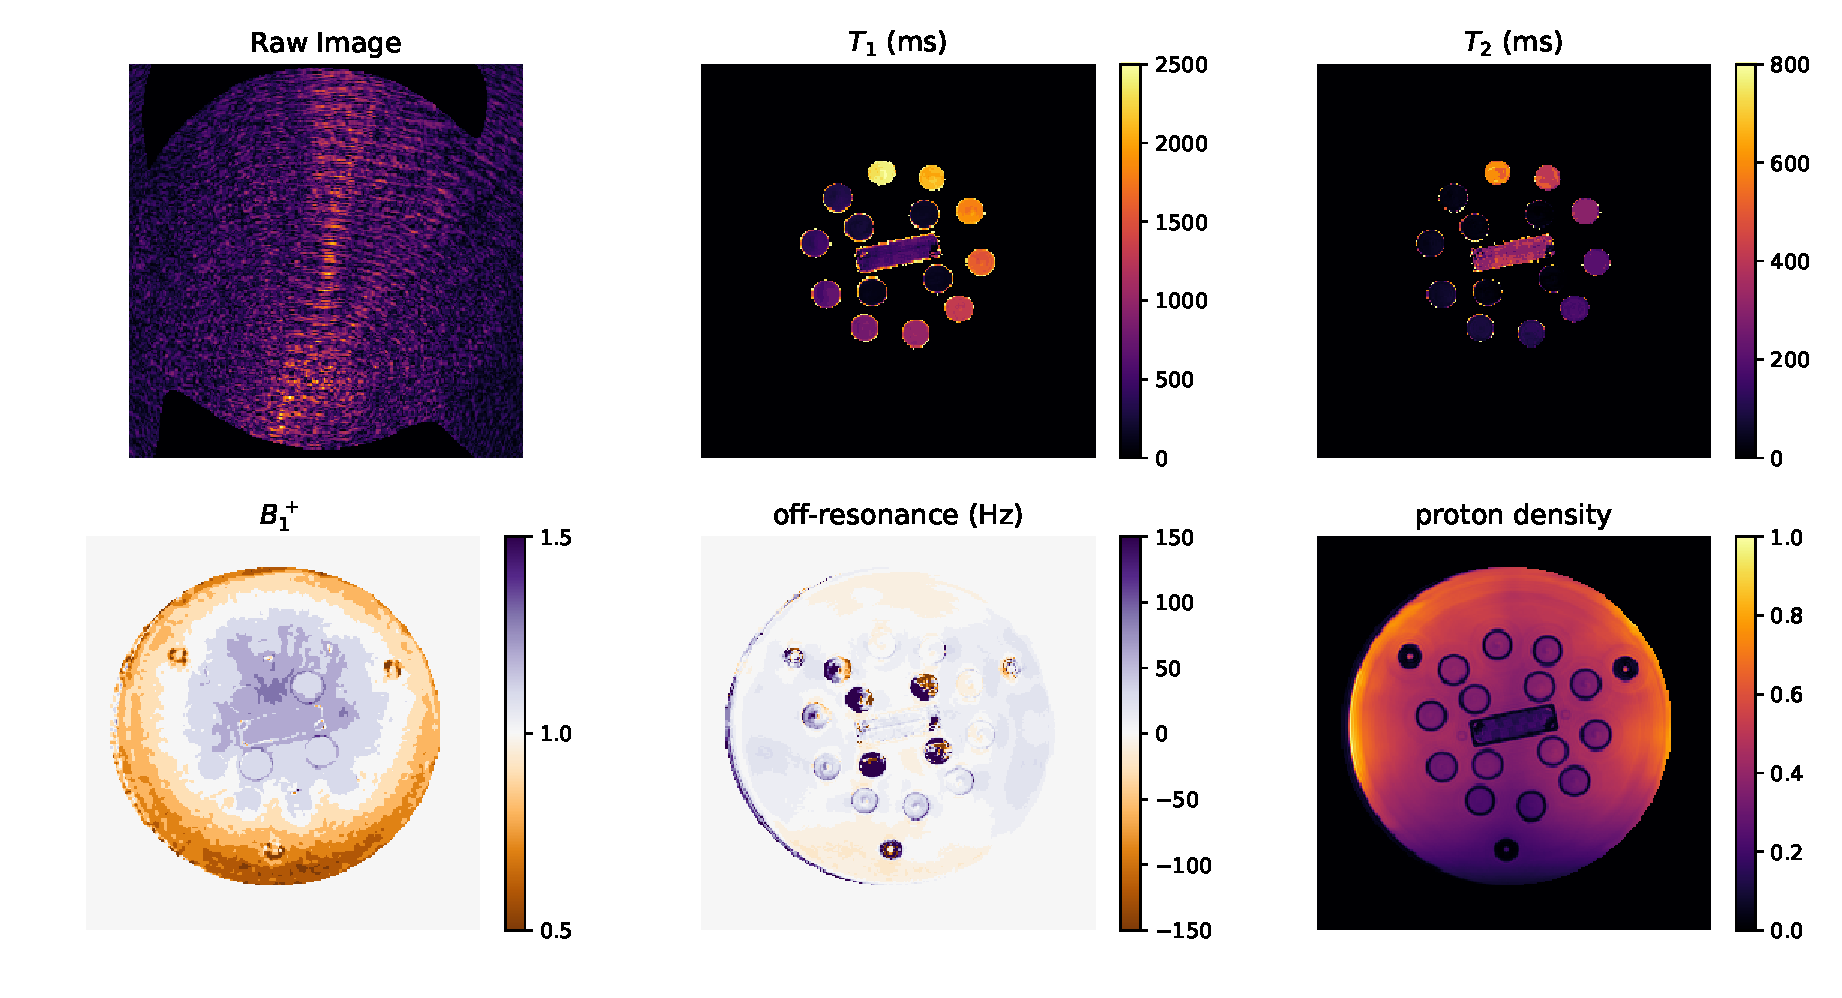
\includegraphics[width=1\textwidth]{img/intro/mrfmap.eps}
\caption{通过模板匹配重建的参数图。}
\label{fig:mrfmap}
\end{figure}
通过简单的计算可以看出,模板匹配的计算复杂度为$O(NL^2K)$。一般来说,MRF信号的时间点$L$通常在1,000以上,字典的个数通常在10,000以上,而体素的个数也会达到10,000以上。所以模板匹配所消耗的时间长,使用MALTAB软件在CPU上运行通常需要几十分钟甚至几小时。因此,虽然模板匹配的方法可以精确地重建参数图,在临床中需要更快速的方法来重建参数图。

第二类方法是降维的思想,先对字典或者数据进行降维处理,然后在降维后的字典和数据上进行匹配。这类方法本质上是对模板匹配的近似。Cauley\cite{groupingmrf}等利用了分组(grouping)的思想进行MRF参数图重建。算法先将字典中的原子分成若干组,使得组内的原子高度相关,并且用组内所有原子的均值来表示这个组的指纹信号,然后再将指纹数据与分组之后的字典进行匹配。该算法大大加速了字典匹配的速度,但是由于依然需要生成字典,字典生成的时间并没有减少。McGivney\cite{svdmrf}等人提出了利用奇异值分解(singular value decomposition, SVD)的方法将字典和指纹数据投影到一个低维子空间,并在子空间中进行匹配。这个方法本质上是压缩了时间方向的维度$L$,从而提高了运算速度。但是这种方法依然需要生成和存储字典,并且相比于模板匹配存在重建误差。

第三类方法是将压缩感知理论应用到MRF中,在重建模型中给参数图加上一些先验信息,以此提高MRF的重建效果。Davies\cite{davies2014compressed}等给出了使用压缩感知进行MRF重建的一般框架,将信号的Bloch响应流型描述成连续信号,并在这个流型上进行下采样。Cline\cite{cline2017air}等改进了Davies的模型,将$B_0$先验信息加入到了模型中,并用基于压缩感知的迭代算法求解模型。Pierre\cite{multiscale}等提出了迭代多尺度MRF重建算法。该方法利用了k-space的先验信息,在数据项和模式识别之间迭代计算直到收敛。Wang\cite{wang2016magnetic}等使用了基于小波变换的压缩感知框架对指纹数据的每一帧进行估计,然后再将重建后的图像和字典进行匹配。Zhao等\cite{zhao2016maximum}利用统计学框架对组织参数进行最大似然估计。在MRF中,对比度加权图像,即指纹图像$X\in \mathbb{C}^{N\times L}$可以被参数化为:
\begin{equation}
	X_l=\phi_l(T_1,T_2)\rho,
\end{equation}
其中$l=1,...,L$,$\rho$为质子密度,$T_1$和$T_2$分别为纵向弛豫时间和横向弛豫时间矩阵,$\phi_l(\cdot)$为第n次采集时的对比度加权函数。于是,图像采集可以被建模为:
\begin{equation}
	B_l=AX_l+\epsilon_l=A\phi_l(T_1,T_2)\rho+\epsilon_l.
\end{equation}
则MRF重建的过程即为从高度下采样的数据$B_l$中估计参数$\{T_1,T_2,\rho\}$的过程。给定上述方程和噪声特征,重建问题可以被建模为如下极大似然估计问题:
\begin{equation}
	\{\hat{T_1},\hat{T_2},\hat{\rho}\}=\argmin_{T_1,T_2,\rho}\sum_{l=1}^L\|B_l-A\phi_l(T_1,T_2)\rho\|_2^2.
\end{equation}
该模型可以提高参数估计的精度并减少采集时间。综合以上方法可以看出,基于压缩感知的MRF重建在一定程度上取得了良好的效果,主要体现在减少采集时间和提高参数图的精度。

最后一大类方法是利用深度学习的框架来重建参数图。Cohen\cite{cohen2018mr}等利用全连接网络(fully connected neural network, FCNN)来训练和重建参数图, Hoppe\cite{hoppe2017deep}和Fabian\cite{balsiger2018magnetic}等构建了MRF的卷积神经网络。虽然这些深度神经网络取得了一定的效果,但是由于网络均使用了监督学习方法,训练所需的真实值依旧由模板匹配生成。因此,网络学习的效果也取决于模板匹配的准确性。

综上所述,MRF参数图的重建需要在精度与速度之间寻求平衡。模板匹配是最基本的重建方法,重建的参数图的精度最高,但是计算比较耗时。降维和深度学习的方法提高了重建的速度,但重建的参数图不可避免地存在误差,而且没有解决字典生成速度慢的问题。压缩感知的方法可以减少扫描时间,但其重建的参数图同样误差偏高。

\subsection{本节小结}
本节主要回顾了磁共振指纹的研究现状。磁共振指纹有三个部分,分别为数据采集、字典生成和模式识别。目前磁共振指纹的瓶颈在于字典生成和匹配的速度慢,使用降维、压缩感知或者深度学习的方法会使得参数图的精度下降。因此,如何在保证参数图精度的前提现提高MRF的重建速度是临床上亟待解决的问题。

\section{本文的主要研究内容和章节安排}
加快MR成像速度一直是临床中十分重要的问题,而基于压缩感知理论的MR成像有着很好的重建效果,并且具有完善的理论分析。MRF是新的量化MRI的方法,可以在单次扫描中同时得到多个组织参数。本文讨论的重点是基于压缩感知的动态重建和基于GPU的MRF字典生成与参数图重建。

第二章,我们首先简单回顾MR成像的基本概念,包括射频场、梯度场、驰豫、k-space和MR序列等。这些内容与MR重建有着密切的联系,了解MR的成像过程可以更深入理解基于压缩感知的MR重建模型与MRF采样和匹配的过程。最后我们给出了EPG模型的数学推导过程,这对有助于我们理解MRF字典的生成。

第三章,针对动态MR图像,利用压缩感知和图像分解的思想,提出了基于二阶时空TGV和核范数的重建模型。模型将图像分解为低秩部分和稀疏部分,其中低秩部分用核范数约束,稀疏部分用二阶时空TGV约束。核范数用来建模动态图像中时间方向高度相关的背景部分,并且可以很好地去除空间伪影;而TGV泛函用来表示图像中的光滑部分,可以在保证重建图像边界清晰的同时减少重建图像中的阶梯效应。我们利用Primal-Dual算法来求解模型,并给出了保证算法收敛的范数估计。为了减少算法的计算时间,我们也利用了图形处理单元来加速MRTLAB程序。我们针对体模、心脏灌注与胸部DCE-MRI图像,对比了四种最前沿的针对动态MR重建模型在不同采样模式和不同采样率下的表现。实验结果表明,相对于其他四个模型,我们提出的模型在不同采样模式和不同采样率下,可以更好地消除空间伪影并且保证图像边缘的清晰,对于胸部DCE-MRI图像尤其显著。

第四章,针对胸部DCE-MRI图像,我们比较了5种不同的时间方向的稀疏项,并对重建结果进行了定量分析。这5种稀疏项分别为Fourier变换、Haar小波变换、二阶TGV和核范数。所有模型均使用FISTA快速算法进行求解。实验结果表明,核范数可以得到最高的信噪比,而TV/二阶TGV可以得到最精确地定量分析。因此,对于胸部DCE-MRI, 选择TV/二阶TGV作为稀疏项可以更好地重建病灶部分,而选择核范数则可以提高图像的整体信噪比。

第五章,针对MRF字典生成与匹配速度慢的问题,我们使用图形处理单元来进行字典生成和模板匹配,并开发了一款开源程序snapMRF。snapMRF可以快速并准确地重建参数图,并且适用于不同的 MRF序列。相比于其他MRF开源程序,snapMRF的字典生成速度提高了10--1000倍, 字典匹配速度提高了10--100倍。







